\documentclass[pdflatex,sn-mathphys-num]{sn-jnl}

\usepackage{graphicx}
\usepackage{multirow}
\usepackage{amsmath,amssymb,amsfonts}
\usepackage{amsthm}
\usepackage[title]{appendix}
\usepackage{xcolor}
\usepackage{textcomp}
\usepackage{manyfoot}
\usepackage{booktabs}
\usepackage{algorithm}
\usepackage{algorithmicx}
\usepackage{algpseudocode}
\usepackage{listings}
\usepackage{tikz}
\usetikzlibrary{arrows.meta,positioning}

\graphicspath{{figs/}{./figs/}{./}}
\setkeys{Gin}{draft=false}

\raggedbottom

\AtBeginDocument{%
  \addtolength{\oddsidemargin}{\evensidemargin}%
  \setlength{\oddsidemargin}{0.5\oddsidemargin}%
  \setlength{\evensidemargin}{\oddsidemargin}%
}

\hypersetup{bookmarksdepth=3}

\AtBeginDocument{%
  \let\snOrigThebibliography\thebibliography
  \renewcommand{\thebibliography}[1]{%
    \snOrigThebibliography{#1}\sloppy\hbadness=10000\relax}%
}

\begin{document}

\title[Wavelet Denoising and Transferred Architectures for Cough Detection]{Wavelet
Denoising Before Spectrogram Extraction Improves Cough Detection for Moderate
Capacity Networks but Not for Densely Connected Ones}

\author[1]{\fnm{Akhilesh Bharadhwaj} \sur{S}}\email{akhilesh.bharadhwaj2024@vitstudent.ac.in}

\author[1]{\fnm{Vishnuvarthan} \sur{M}}\email{vishnuvarthan.m2024@vitstudent.ac.in}

\author[1]{\fnm{Nithin} \sur{Kumar}}\email{nithinkumar.j2024a@vitstudent.ac.in}

\author[1]{\fnm{Ajay} \sur{Pokkali}}\email{ajay.pokkali2024@vitstudent.ac.in}

\author*[1]{\fnm{Ravi} \sur{Tiwari}}\email{ravi.tiwari@vit.ac.in}

\affil*[1]{\orgdiv{School of Electronics Engineering (SENSE)},
  \orgname{Vellore Institute of Technology},
  \orgaddress{\city{Chennai}, \state{Tamil Nadu}, \country{India}}}

\abstract{Automatic detection of coughs in continuously recorded audio is the
gating step for any acoustic respiratory screening system, and its reliability
determines how often such a system raises an alarm on material that contains no
cough at all. We study that step on crowdsourced recordings, where background
noise varies without constraint, and we examine three design choices
together: whether the network receives a linear or a perceptually scaled
spectrogram, whether the waveform is denoised with a wavelet transform before
the spectrogram is formed, and which convolutional architecture performs the
classification. Four models are evaluated, a compact network trained from
scratch and three architectures transferred from a large image corpus, each
with and without denoising, giving eight configurations measured on an
identical partition of 4,577 held out recordings. Perceptual frequency scaling
improves every architecture it is applied to. Denoising helps the two models
of moderate capacity, raising the best accuracy to 96.53 percent with a
precision of 97.59 percent and a recall of 97.31 percent, but it does not help
the densely connected network, whose accuracy is unchanged within rounding. We
also recover the full error structure of every configuration from the reported
rates and show that the class imbalance of the corpus conceals a wide spread
in specificity, from 90.84 to 95.73 percent, that plain accuracy does not
reveal. Ranking the configurations by balanced accuracy preserves the
conclusion while narrowing the apparent margins considerably, and we report
the reordering this causes because it changes which model a deployment should
prefer.}

\keywords{Respiratory screening, Acoustic event detection, Crowdsourced audio,
Perceptual frequency scaling, Class imbalance, Signal preprocessing}

\maketitle

\section{Introduction}\label{sec:intro}

A cough is one of the few symptoms that produces a signal a microphone can
capture without contact, without a clinician present and without the person
being examined doing anything beyond carrying a telephone. That property has
made acoustic analysis of coughing an attractive route to population scale
respiratory screening, and the interest intensified during the COVID-19
pandemic, when the need to triage large numbers of people quickly exceeded the
capacity of testing programmes in most countries. Systems built in that period
sought to infer disease status directly from a recorded cough, and several
reported encouraging results on data gathered through web forms and mobile
applications~\cite{brown2020, imran2020, laguarta2020}. The conditions of the
pandemic also produced the open corpora that made comparison across research
groups possible, of which the COUGHVID collection is among the
largest~\cite{orlandic2021}.

Beneath the question of what a cough reveals lies a prior question that is
easier to state and harder to dismiss: is the sound a cough at all. Every
screening pipeline that operates on continuous audio must first decide which
segments contain coughing and which contain speech, laughter, door closures,
traffic, music or silence. That decision is the gate through which all later
inference passes. A missed cough removes a person from consideration entirely,
and a false detection sends noncough audio into a disease classifier that was
never trained on it, producing an output with no meaning that is nonetheless
reported with a confidence value. In a screening context the second error is
the more insidious, because it generates referrals that consume clinical time
and erode confidence in the system among the people who have to act on its
output. Detection therefore deserves to be studied as a problem in its own
right rather than as a preprocessing detail, and that is the subject of this
paper.

The acoustic properties of a cough make the detection problem tractable in
principle. A cough is a forced expiratory manoeuvre with a characteristic
three phase structure: an explosive onset as the glottis opens against raised
subglottal pressure, an intermediate phase of rapid airflow, and a voiced or
unvoiced termination. The onset produces a broadband transient with energy
extending well above the range occupied by conversational speech, and the
sequence of phases gives a temporal envelope that is distinctive even when the
spectrum alone is ambiguous. Early systems exploited exactly these properties
through features designed by hand, including Mel frequency cepstral
coefficients, spectral centroid, zero crossing rate and short term energy,
often with a classifier of modest capacity on
top~\cite{swarnkar2013, hoyosbarcelo2018, mongealvarez2019}. Such features are
interpretable and inexpensive, and they remain appropriate where computation is
severely constrained, but they encode a fixed prior about what distinguishes a
cough and they generalise poorly when recording conditions depart from those
the designer anticipated.

Learned representations displaced designed ones for the same reasons they did
elsewhere in audio processing. Presenting a time frequency image to a
convolutional network allows the network to discover which regions of the
plane carry discriminative information, and work on general audio event
recognition established both that this approach is effective and that
architectures developed for natural images transfer to it with little
modification~\cite{piczak2015, hershey2017, salamon2017}. The transfer is
possible because a spectrogram, once rendered as an image, exhibits the local
structure that convolutional kernels are suited to, and because large image
corpora supply initial filters that are generic enough to be useful on inputs
quite unlike photographs~\cite{deng2009, pan2010}. The practical consequence is
that a cough detector can be built from an architecture trained on millions of
images, retrained on a corpus of a size that a research group can actually
assemble.

Two choices within that recipe are usually made without being examined.
The first concerns the frequency axis of the spectrogram. A short time
Fourier transform spaces its bins linearly, which allocates the same
resolution to the region between 7 and 8~kHz as to the region between 100 and
200~Hz, although the latter carries far more of what distinguishes one
respiratory sound from another. Mapping the axis onto a perceptual scale
redistributes that resolution, compressing the upper range and expanding the
lower, following the relationship established in early work on speech
features~\cite{davis1980}. The second concerns noise. Crowdsourced recordings
are made on unknown equipment in uncontrolled surroundings, so the corpus
contains traffic, electrical hum, wind, television audio and clipping, none of
it labelled. Wavelet decomposition offers a principled way to attenuate such
interference before any spectrogram is formed, because it represents a signal
at multiple resolutions simultaneously and allows the components that carry
broadband transient energy to be separated from those that do
not~\cite{mallat1989}, with thresholding rules that have a firm statistical
basis~\cite{donoho1994, donoho1995}.

Whether denoising is worth performing is less obvious than it first appears,
and the reason is that it interacts with the capacity of the network placed
after it. A deep network with extensive feature reuse may already learn
representations that ignore interference, in which case removing that
interference beforehand buys nothing and risks discarding genuine high
frequency content that the network had learned to exploit. A network of more
modest capacity, or one trained for fewer epochs, may lack that ability and
benefit substantially. This interaction is rarely tested, because most studies
fix one architecture and vary the preprocessing, or fix the preprocessing and
vary the architecture, so the question of whether the benefit of denoising
depends on what follows it remains open. The present work tests precisely that
interaction by crossing both factors on one corpus with one partition.

This paper makes the following contributions.

\begin{enumerate}
\item We evaluate eight configurations on an identical partition of the
COUGHVID corpus, crossing two spectrogram representations and the presence or
absence of wavelet denoising across four convolutional architectures, so that
the effect of each factor can be read without the confound of a differing
split or a differing training budget.
\item We show that the benefit of wavelet denoising depends on the
architecture that follows it. The two models of moderate capacity gain, by
0.77 and 0.35 accuracy points respectively, whereas the densely connected
network does not, its accuracy changing by less than one tenth of a point in
the opposite direction.
\item We recover the complete confusion structure of all eight configurations
from the published rates and the composition of the test partition, and report
specificity and balanced accuracy, neither of which the accuracy figure alone
exposes on a corpus whose classes stand in a ratio greater than two to one.
\item We show that ranking by balanced accuracy preserves the identity of the
best configuration but compresses the margins between the remainder and
reorders the models in the middle of the table, and we set out what this
implies for a deployment that must choose between a stronger detector and a
smaller one.
\end{enumerate}

The remainder of the paper is organised as follows.
Section~\ref{sec:related} reviews the relevant literature and identifies the
gap addressed here. Section~\ref{sec:design} specifies the processing pipeline
and the four architectures. Section~\ref{sec:setup} describes the corpus, the
training configuration, the metrics and the information needed to repeat the
work. Section~\ref{sec:results} presents the results, the recovered error
structure and the limitations of the study. Section~\ref{sec:conclusion}
concludes.

\section{Related work and its limitations}\label{sec:related}

This section reviews five strands of work and states what each leaves
unresolved. Section~\ref{sec:rel-handcrafted} covers detection from features
designed by hand. Section~\ref{sec:rel-corpora} covers the open corpora that
made comparative evaluation possible and the screening systems built on them.
Section~\ref{sec:rel-transfer} covers spectrogram inputs and transferred
architectures. Section~\ref{sec:rel-eval} covers evaluation practice in this
literature and why reported figures are difficult to compare across studies.
Section~\ref{sec:rel-denoise} covers denoising for respiratory audio and
states the gap this study addresses.

\subsection{Detection from designed features}\label{sec:rel-handcrafted}

The first generation of automatic cough detectors described the signal through
a small set of quantities chosen for their physical interpretation and passed
them to a classifier of modest capacity. Swarnkar and colleagues separated wet
from dry coughs in paediatric patients using features of this kind, showing
that the distinction clinicians draw by ear has a measurable acoustic
correlate~\cite{swarnkar2013}. Hoyos-Barcel\'o and colleagues addressed the
engineering problem directly, implementing a nearest neighbour classifier
efficiently enough to detect cough events on a smartphone in real
time~\cite{hoyosbarcelo2018}, and the same group later described a detector
built on local moments computed over the time frequency
plane~\cite{mongealvarez2019}. Nemati and colleagues considered the broader
task of distinguishing cough types rather than merely detecting
them~\cite{nemati2019}.

The features themselves were chosen to reflect properties of the signal that
can be described in words. Cepstral coefficients summarise the gross shape of
the spectral envelope in a small number of values and so capture the resonant
structure imposed by the airway. Spectral centroid locates the centre of mass
of the spectrum and separates sounds that are bright from those that are
dull. Zero crossing rate responds to the proportion of high frequency content
and distinguishes the noisy portion of a cough from voiced material. Short
term energy traces the envelope and therefore the phase structure that gives
a cough its characteristic shape in time. A classifier presented with these
quantities is working with a compact description that a clinician can be
shown and, in principle, dispute.

These systems share two strengths that are easy to undervalue. They are cheap
enough to run continuously on battery powered hardware, and their decisions
can be traced to quantities a clinician can be shown. Their weakness is that
the feature set encodes an assumption about what a cough sounds like, fixed
before any data is seen. Where the recording conditions match that assumption
the systems perform well; where they do not, performance falls in ways that
cannot be corrected by retraining the classifier alone, because the
information the classifier would need has already been discarded by the
feature extractor. Crowdsourced audio departs from any fixed assumption by
construction, which is what motivated the move to learned representations.

\subsection{Open corpora and screening systems}\label{sec:rel-corpora}

Progress in this area was limited for a long period by the absence of data
that different groups could share. The pandemic changed that. Brown and
colleagues assembled crowdsourced respiratory recordings and showed that
simple classifiers applied to them could separate reported COVID-19 cases from
controls at rates well above chance~\cite{brown2020}. Sharma and colleagues
released the Coswara database, covering breathing, cough and voice
together~\cite{sharma2020}. Orlandic and colleagues released COUGHVID, the
corpus used here, and documented both its scale and the variability that makes
it demanding: the recordings arrive through a web interface from unknown
devices in unknown surroundings, and a substantial fraction contain no cough at
all~\cite{orlandic2021}.

Screening systems followed quickly. Imran and colleagues built a deployable
application around a deep classifier operating on cough
audio~\cite{imran2020}, Laguarta and colleagues reported that a model trained
on cough recordings alone could discriminate COVID-19 status~\cite{laguarta2020},
Pahar and colleagues examined the same question across smartphone recordings
gathered globally~\cite{pahar2021}, and Coppock and colleagues trained a
network end to end on breath and cough audio~\cite{coppock2021}. Later work
pursued architectural refinement for the same task~\cite{dentamaro2022,
vijayakumar2021, lella2021}, and independent groups revisited the crowdsourced
data to test how far the early claims
generalised~\cite{son2022}. Ijaz and colleagues survey the field as a
whole~\cite{ijaz2022}.

A reckoning followed the first wave of results. Several of the early claims
rested on corpora in which the positive and negative groups differed in more
than their disease status, because the people who contributed them were
recruited through different channels, recorded in different circumstances and
sometimes on different classes of device. A model can separate such groups
without learning anything about respiratory disease, and independent
re examination of crowdsourced material has reported figures below those
initially announced once such confounds are controlled~\cite{son2022}. The
episode left the field with a sharper sense of what an acoustic screening
claim requires: a negative class drawn from the same population and the same
recording conditions as the positive one, a partition that separates
contributors rather than recordings, and a baseline that shows what the
prior alone would achieve.

That history bears directly on the detection problem studied here, because a
detector is the component that decides which audio a disease model ever sees.
If detection errors correlate with recording conditions, and crowdsourced
recording conditions correlate with contributor, then a detector can
introduce exactly the kind of confound the field has learned to guard
against, before the disease model is reached at all.

The limitation relevant here is one of emphasis rather than of method. Almost
all of this work takes the presence of a cough as given and asks what the
cough indicates. The recordings are segmented, often manually or with a
detector whose own error rate is not reported, and the screening model is
evaluated on the segments that survive. Any error introduced at that stage is
therefore absent from the reported figures while remaining present in any
deployment, and since the detection stage is where noncough audio is rejected,
its false positive rate propagates directly into the referral rate of the
complete system.

\subsection{Spectrogram inputs and transferred architectures}\label{sec:rel-transfer}

Treating a time frequency representation as an image allows a convolutional
network to learn its own features, and the approach was established on general
audio before it was applied to respiratory sounds. Piczak showed that a
convolutional network on spectrogram inputs is competitive for environmental
sound classification~\cite{piczak2015}, Salamon and Bello improved the result
with augmentation designed for audio~\cite{salamon2017}, and Hershey and
colleagues examined how image architectures behave at large scale on
audio~\cite{hershey2017}, supported by the release of a correspondingly large
labelled collection~\cite{gemmeke2017}.

The architectures themselves originate in image recognition. Residual
connections allowed networks to be made substantially deeper without the
degradation that had previously accompanied depth~\cite{he2016}. Dense
connectivity, in which every layer receives the feature maps of all preceding
layers, strengthens gradient flow further and encourages features to be reused
rather than recomputed~\cite{huang2017}. Separately, work on efficiency
produced architectures intended for devices with limited memory and power, of
which the inverted residual design with linear bottlenecks is a widely adopted
example~\cite{sandler2018}. All three transfer to spectrogram inputs by
replacing the classification head, with initial weights taken from a large
image corpus~\cite{deng2009}; the general conditions under which such transfer
succeeds are surveyed by Pan and Yang~\cite{pan2010}.

Why transfer from photographs to spectrograms works at all deserves a word,
because the two kinds of image are not alike. A photograph is approximately
stationary under translation in either direction, so a feature is equally
meaningful wherever it appears. A spectrogram is not: translating a pattern
along the time axis leaves its meaning intact, whereas translating it along
the frequency axis changes what it represents. A convolution applied over both
axes therefore imposes an invariance on the frequency axis that the signal
does not possess. Transfer nonetheless succeeds, and the reason appears to be
that the early layers of an image network learn generic detectors of edges,
corners and oriented texture, and these remain useful on a spectrogram because
the structures that matter there, harmonic ridges, broadband vertical
transients and the boundaries of energy bursts, are themselves edges and
textures. The layers whose features are specific to natural images lie deeper,
and those are the layers that retraining adjusts.

What is less often examined is the frequency axis these architectures receive.
A linear axis and a perceptually scaled one present the same recording as
visibly different images, and the convolution kernel, which is spatially
uniform, therefore sees a different problem in each case. The perceptual
mapping concentrates resolution where respiratory sounds differ most, and the
relationship used for it was established in the speech recognition
literature~\cite{davis1980}. The choice also interacts with the resize that
precedes a transferred network, since an architecture expecting a square
input of fixed size will compress or stretch whatever representation it is
given, and the amount of distortion this introduces depends on how many
frequency bins the representation carried in the first place. Studies
comparing the two axes on cough detection specifically, with everything else
held constant, are uncommon.

\subsection{Evaluation practice in this literature}\label{sec:rel-eval}

Reported figures in cough analysis are difficult to compare across studies,
and the reasons are worth setting out because they shape how the present
results should be read.

The first reason is that the corpora differ in what they contain. A corpus
assembled from clinical recordings contains coughs produced by people who are
unwell, captured on consistent equipment at a controlled distance. A
crowdsourced corpus contains coughs produced on request by a largely healthy
population on whatever device they happened to hold, at distances and levels
that vary by orders of magnitude, with background content that ranges from
silence to television audio. Detection is a different problem in the two
settings, and a figure obtained in one does not transfer to the
other~\cite{orlandic2021, ijaz2022}. The same applies to the negative class.
What counts as a noncough recording is defined differently by different
collections, and a detector evaluated against a negative class consisting
mostly of speech will report a different error rate from one evaluated
against a negative class dominated by mechanical noise.

The second reason is the partition. Many reported results use a random split
at the level of the recording, which allows multiple recordings from one
contributor to appear on both sides of the division. Where contributors
differ systematically in device, room and vocal character, such a split lets
a model recognise the contributor rather than the event, and the resulting
figure overstates what the model would achieve on an unseen person. Splitting
by contributor avoids this but is possible only where contributor identifiers
are retained, which not every collection provides.

The third reason is the choice of summary measure. Cough corpora are commonly
imbalanced, and on an imbalanced partition accuracy is dominated by the
majority class, so two systems with identical accuracy can differ
substantially in how they distribute their errors. Precision, recall and
$F_1$ expose that distribution, which is why all four are reported here,
and the balance between them is the quantity a deployment actually
selects on. Comparable studies vary in which subset they report, and a study
reporting accuracy alone leaves a reader unable to tell whether an
improvement came from detecting more coughs or from rejecting more noncough
material~\cite{son2022}.

The consequence for the present work is methodological rather than
substantive. Because cross study comparison is unreliable for these reasons,
the design adopted here holds the corpus, the partition, the optimiser and the
evaluation fixed and varies only the two factors under examination. The
comparisons that carry the argument are therefore internal to this study, and
we draw no conclusion from the numerical proximity of our figures to those
reported elsewhere.

\subsection{Denoising for respiratory audio, and the gap}\label{sec:rel-denoise}

Wavelet analysis is well matched to signals whose informative content is
transient. Decomposing a waveform across scales isolates abrupt broadband
events, such as the explosive onset of a cough, from interference that is
either narrowband or slowly varying, and the multiresolution framework that
makes this possible is due to Mallat~\cite{mallat1989}. The statistical basis
for discarding coefficients was established by Donoho and Johnstone, who showed
that thresholding in a wavelet basis is near optimal for recovering a signal
from additive noise~\cite{donoho1994} and characterised the behaviour of soft
thresholding in particular~\cite{donoho1995}. Applied to a cough recording, the
approach attenuates the background while leaving the transient structure that
carries the discriminative information largely intact.

Reported results on respiratory audio generally favour denoising, but the
evidence has a consistent shape that limits what can be drawn from it. A study
fixes one architecture, applies denoising, observes an improvement and
concludes that denoising is beneficial. This establishes that denoising helps
that architecture on that corpus. It does not establish that the benefit is a
property of denoising rather than of the pairing, and there is a specific
reason to doubt that it is. Denoising and architectural capacity address the
same problem by different means. Removing interference before the network sees
it, and building a network able to ignore interference, are substitutes rather
than complements, so a network that already achieves invariance through its own
structure should gain little from preprocessing and may lose whatever genuine
high frequency content the preprocessing removes along with the noise.

The gap this study addresses follows directly. We hold the corpus, the
partition, the optimiser and the evaluation fixed, and vary the representation
and the denoising across four architectures that differ substantially in depth
and in the mechanism by which they reuse features. This design allows the
question to be posed as an interaction rather than as a main effect, and
Section~\ref{sec:results} shows that the interaction is real: the benefit of
denoising is not a constant of the method but depends on what is placed after
it.

\section{System design}\label{sec:design}

This section specifies the processing chain in the order a recording passes
through it, and then the four classifiers placed at its end.
Section~\ref{sec:d-overview} gives the shape of the pipeline and fixes
notation. Section~\ref{sec:d-cond} covers audio conditioning.
Section~\ref{sec:d-wav} develops the wavelet denoising stage.
Section~\ref{sec:d-spec} covers the two spectrogram representations.
Section~\ref{sec:d-arch} describes the four architectures, and
Section~\ref{sec:d-why} states why this particular set was chosen.

\subsection{Overview and notation}\label{sec:d-overview}

Let $x[n]$ denote a recording sampled at rate $f_s$, and let
$y \in \{\text{cough}, \text{noncough}\}$ denote the label to be predicted.
The pipeline applies four operations in sequence. The waveform is brought to a
common sampling rate and channel count; it is optionally denoised in a wavelet
basis; it is converted to a time frequency image; and the image is classified.
Figure~\ref{fig:pipeline} shows the arrangement, including the branch point at
which the two spectrogram representations diverge and the optional stage whose
contribution is the question this paper poses.

The optional stage is what makes the design a factorial one rather than a
single pipeline. Writing $\mathcal{W}$ for the denoising operator,
$\mathcal{S}$ for the spectrogram operator and $g_\theta$ for a classifier
with parameters $\theta$, the eight configurations evaluated in
Section~\ref{sec:results} are
\begin{equation}
\hat{y} = g_\theta\big(\mathcal{S}(\mathcal{W}^{\,\delta}(x))\big),
\qquad \delta \in \{0, 1\},
\label{eq:config}
\end{equation}
with $\delta = 1$ indicating that denoising is applied and $\delta = 0$ that
it is bypassed, and with $\mathcal{S}$ and $g_\theta$ ranging over the
representations and architectures described below. Holding everything outside
Equation~\eqref{eq:config} fixed is what allows the effect of $\delta$ to be
attributed to denoising rather than to an incidental difference in the
experimental conditions.

\begin{figure}[t]
\centering
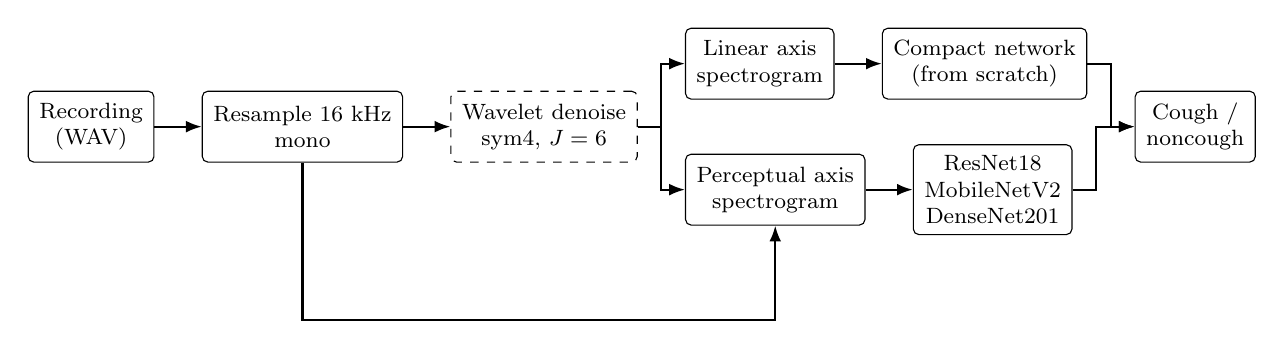
\begin{tikzpicture}[
  node distance=6mm,
  box/.style={draw, rounded corners=2pt, align=center, inner sep=4pt,
              minimum height=9mm, font=\footnotesize},
  opt/.style={box, dashed},
  ar/.style={-{Latex[length=2mm]}, thick}
]
\node[box] (wav) {Recording\\(WAV)};
\node[box, right=of wav] (rs) {Resample 16~kHz\\mono};
\node[opt, right=of rs] (wd) {Wavelet denoise\\sym4, $J=6$};
\node[box, right=of wd, yshift=8mm] (stft) {Linear axis\\spectrogram};
\node[box, right=of wd, yshift=-8mm] (mel) {Perceptual axis\\spectrogram};
\node[box, right=of stft] (cnn) {Compact network\\(from scratch)};
\node[box, right=of mel] (tl) {ResNet18\\MobileNetV2\\DenseNet201};
\node[box, right=of cnn, yshift=-8mm] (out) {Cough /\\noncough};

\draw[ar] (wav) -- (rs);
\draw[ar] (rs) -- (wd);
\draw[ar] (wd.east) -- ++(3mm,0) |- (stft.west);
\draw[ar] (wd.east) -- ++(3mm,0) |- (mel.west);
\draw[ar] (stft) -- (cnn);
\draw[ar] (mel) -- (tl);
\draw[ar] (cnn.east) -- ++(3mm,0) |- (out.west);
\draw[ar] (tl.east) -- ++(3mm,0) |- (out.west);
\draw[ar] (rs.south) -- ++(0,-20mm) -| (mel.south);
\end{tikzpicture}
\caption{Processing chain. The denoising stage is drawn dashed because it is
present in half of the configurations and absent in the other half, which is
the comparison the study is built around. The lower path from the resampling
stage carries the undenoised signal directly to spectrogram extraction.
Beyond the stage order, the figure shows that the two spectrogram
representations are formed from the same conditioned waveform, so any
difference in the results attaches to the frequency axis rather than to
anything earlier.}
\label{fig:pipeline}
\end{figure}

\subsection{Audio conditioning}\label{sec:d-cond}

Recordings arrive at heterogeneous sampling rates and channel counts, and both
are normalised before anything else is done. Files recorded in stereo are
reduced to a single channel by averaging, which preserves content common to
both channels and attenuates anything uncorrelated between them. All material
is then resampled to $f_s = 16$~kHz.

The choice of rate is a compromise between fidelity and cost. A rate of
16~kHz places the Nyquist limit at 8~kHz, which retains the spectral region in
which cough energy is concentrated while discarding content above it, and it
reduces the sample count of a typical recording by roughly two thirds relative
to the 44.1~kHz material that consumer devices commonly produce. The explosive
onset of a cough does deposit some energy above 8~kHz, so the choice is not
free of cost; the justification is that the discriminative information is
dominated by the lower range and that the reduction in sample count propagates
through every subsequent stage, including the wavelet decomposition, whose
cost is linear in signal length.

\subsection{Wavelet denoising}\label{sec:d-wav}

Denoising is performed in a wavelet basis rather than by filtering in the
frequency domain, for a reason specific to the signal. A cough is a transient,
so its energy is localised in time and spread across frequency, which is the
opposite of the profile that a fixed frequency domain filter handles well. A
wavelet basis represents the signal at several resolutions at once and so can
distinguish a short broadband event from sustained interference occupying the
same band, which a filter cannot.

The decomposition expresses the signal as a coarse approximation at level $J$
together with the detail removed at every level above it,
\begin{equation}
x[n] = A_J[n] + \sum_{j=1}^{J} D_j[n],
\label{eq:mra}
\end{equation}
where $A_J[n]$ holds the low frequency content remaining after $J$ successive
halvings of the band and $D_j[n]$ holds the detail at level $j$. Each
level separates the current approximation into a new approximation and a
detail band, so $D_1$ carries the highest frequency octave and $D_J$ the
lowest of those removed. We set $J = 6$ and use the sym4 wavelet, a member of
the symlet family chosen because it is nearly symmetric, which limits the
phase distortion introduced into the reconstructed transient, and because its
support is short enough to remain localised against events lasting a few tens
of milliseconds.

Denoising proceeds by attenuating detail coefficients whose magnitude is
consistent with noise rather than with signal. The classical treatment fixes
a threshold per level and shrinks each coefficient toward zero by that
amount, discarding those that do not survive the
subtraction~\cite{donoho1994, donoho1995}. The procedure used here is the
empirical Bayesian alternative, which places a mixture prior on the detail
coefficients at each level,
\begin{equation}
d_{j,k} \sim (1 - w_j)\,\delta_0 + w_j\,\gamma,
\label{eq:eb}
\end{equation}
where $\delta_0$ is a point mass at zero, $\gamma$ is a heavy tailed Cauchy
density and the mixing weight $w_j$ is estimated from the coefficients at
level $j$ by marginal maximum likelihood. Each coefficient is then replaced
by the median of its posterior distribution~\cite{johnstone2005}. Because
$w_j$ is estimated separately at every level, the amount of shrinkage adapts
to how much of the energy at that scale is attributable to noise instead of
being set by one global rule, and the heavy tail of the prior leaves large
coefficients close to unshrunk. The signal is reconstructed from the retained
approximation and the shrunken details.

Figure~\ref{fig:denoise} shows the operation on one cough and one noncough
recording, each at three stages. Reading across the top row establishes that
the transient structure of the cough survives the operation, which is the
property the stage must have if it is to be useful; reading down the third
column compares what was discarded in the two cases, which is where the two
classes differ most visibly.

\begin{figure}[t]
\centering
\begin{tabular}{@{}ccc@{}}
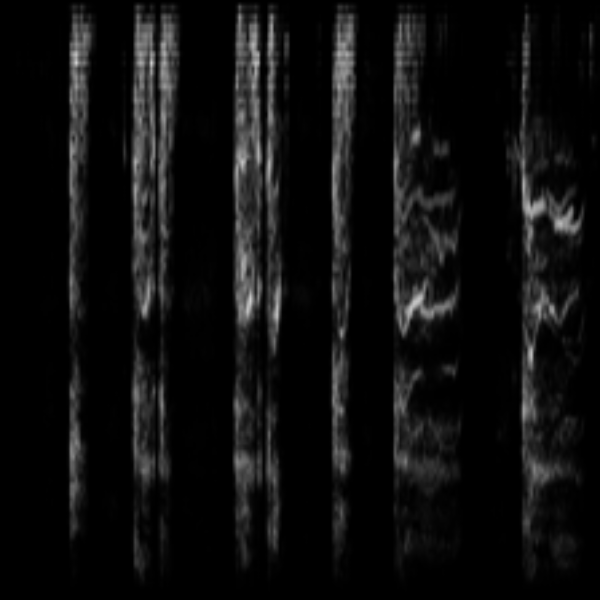
\includegraphics[width=0.30\textwidth]{denoise_a_cough_raw.png} &
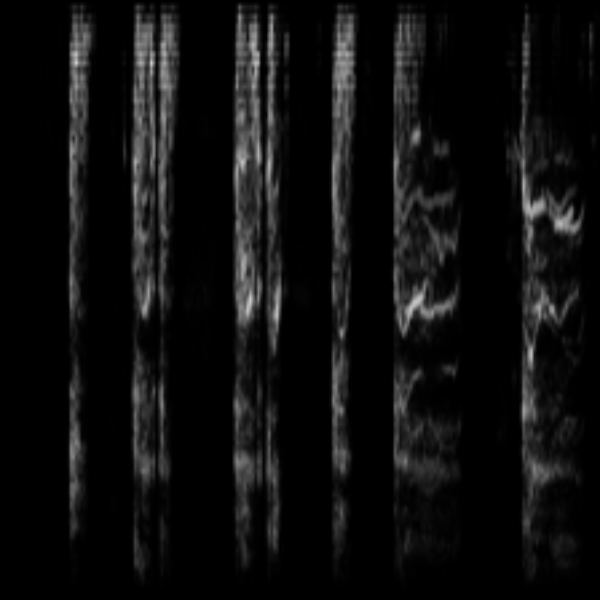
\includegraphics[width=0.30\textwidth]{denoise_b_cough_denoised.png} &
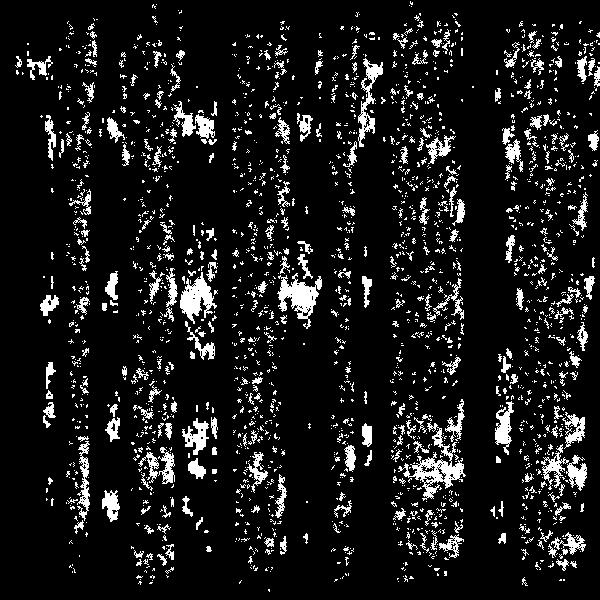
\includegraphics[width=0.30\textwidth]{denoise_c_cough_removed.png} \\[2pt]
{\footnotesize (a) cough, original} &
{\footnotesize (b) cough, denoised} &
{\footnotesize (c) cough, removed} \\[6pt]
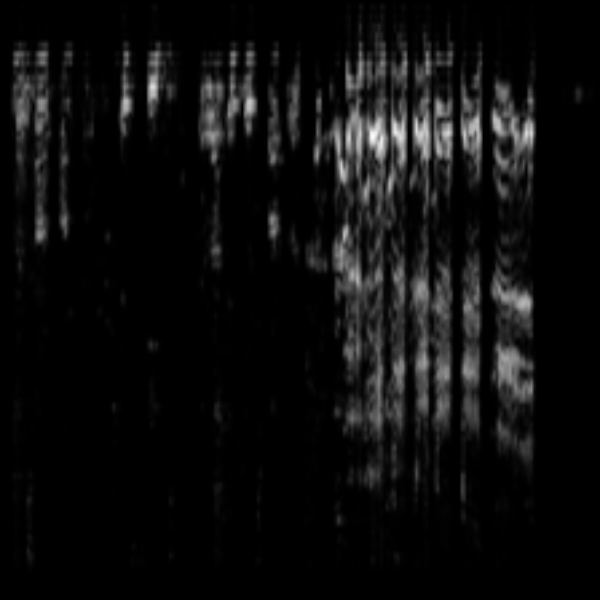
\includegraphics[width=0.30\textwidth]{denoise_d_noncough_raw.png} &
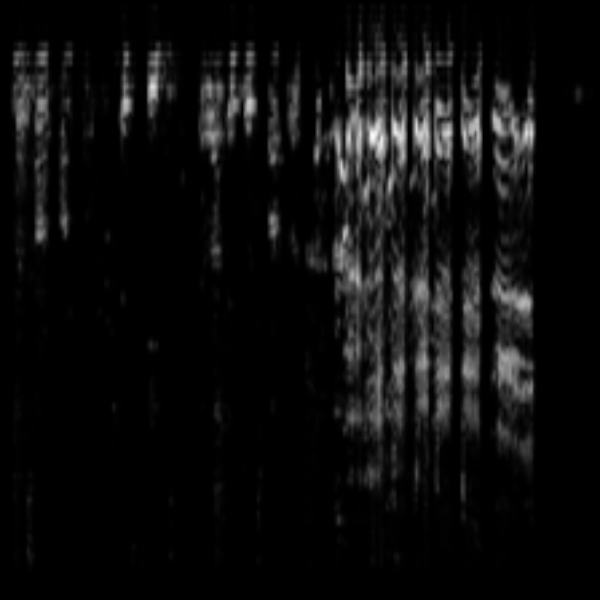
\includegraphics[width=0.30\textwidth]{denoise_e_noncough_denoised.png} &
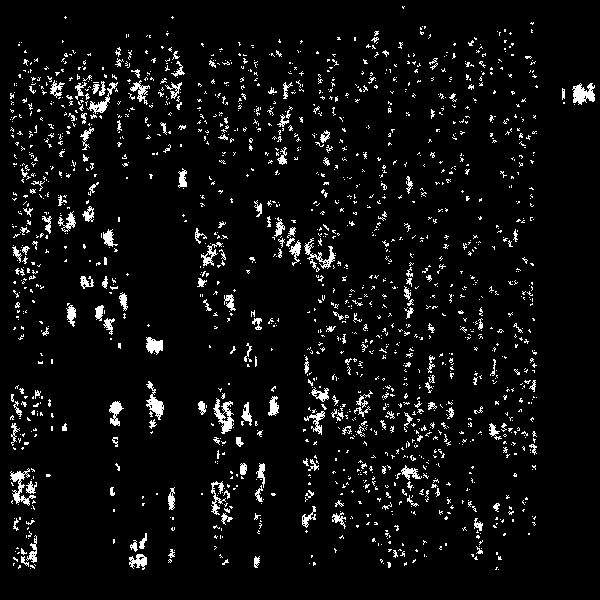
\includegraphics[width=0.30\textwidth]{denoise_f_noncough_removed.png} \\[2pt]
{\footnotesize (d) noncough, original} &
{\footnotesize (e) noncough, denoised} &
{\footnotesize (f) noncough, removed} \\
\end{tabular}
\caption{Effect of the sym4 decomposition at level six on a representative
cough recording, in the top row, and a representative noncough recording, in
the bottom row. Each panel is a time frequency representation, with time on
the horizontal axis and frequency on the vertical. Panels (a) and (d) show
the conditioned input and (b) and (e) the reconstruction after shrinkage. The
dominant transient structure of the cough is preserved from (a) to (b), which
is the property the operation has to have if it is not to suppress the energy
the classifier depends on. Panels (c) and (f) are diagnostic rather than
quantitative: each is the absolute difference between the two images above it,
rescaled to the full display range and amplified to make faint structure
visible. They indicate where in the plane the reconstruction departs from the
input, and that the departure avoids the region carrying the cough transient.
Because each difference panel is rescaled independently of the other, the
intensities in (c) and (f) are not on a common scale and the two panels should
not be compared against each other.}
\label{fig:denoise}
\end{figure}

The level $J = 6$ determines how much of the signal is exposed to shrinkage.
At 16~kHz the sixth level corresponds to an approximation band below roughly
125~Hz, so the decomposition reaches well beneath the range in which cough
energy is concentrated and gives the thresholding access to the bands where
both the transient and the interference reside. A shallower decomposition
would leave low frequency interference untouched in the approximation; a
deeper one would continue subdividing a band that by then contains little but
the recording offset.

\subsection{Spectrogram representations}\label{sec:d-spec}

Both representations begin from the same conditioned waveform and differ only
in how the frequency axis is spaced, which is what allows their comparison to
isolate the effect of that spacing.

\subsubsection{Linear frequency axis}\label{sec:d-stft}

The short time Fourier transform is computed as
\begin{equation}
X(m, k) = \sum_{n} x[n]\, w[n - m]\, e^{-j 2 \pi k n / N},
\label{eq:stft}
\end{equation}
where $m$ indexes the analysis frame, $k$ the frequency bin, $w[\cdot]$ is a
Hamming window and $N$ is the transform length. The magnitude $|X(m,k)|$ is
retained and the phase discarded, since the classifier operates on an image.

The representation preserves the full time frequency structure of the signal
but spaces its bins uniformly, which distributes resolution evenly across the
spectrum. For a cough this allocation is inefficient. The region above 4~kHz
occupies half of the available bins while carrying comparatively little of
what separates a cough from a door closing, and the region below 500~Hz, where
the voiced termination and much of the envelope structure reside, is
represented by a small number of bins. This representation is used for the
baseline network described in Section~\ref{sec:d-cnn}.

\subsubsection{Perceptual frequency axis}\label{sec:d-mel}

The perceptual representation warps the frequency axis according to
\begin{equation}
f_{\mathrm{mel}} = 2595 \log_{10}\!\left(1 + \frac{f}{700}\right),
\label{eq:mel}
\end{equation}
in which $f$ is the physical frequency in hertz and $f_{\mathrm{mel}}$ the
warped value~\cite{davis1980}. The mapping is approximately linear below
about 700~Hz and approximately logarithmic above it, so the low frequency
region is expanded relative to a linear axis and the high frequency region
compressed. A bank of triangular filters spaced uniformly on this warped axis
is applied to the magnitude spectrum, and the filter outputs are converted to
a logarithmic amplitude scale.

Figure~\ref{fig:mel} shows the mapping and the bank it produces. Panel (a)
plots Equation~\eqref{eq:mel} against a linear reference, and the departure
between the two curves is the redistribution of resolution the mapping
performs. Panel (b) shows the consequence for the filters themselves, which
is the quantity that matters for what the network receives.

\begin{figure}[t]
\centering
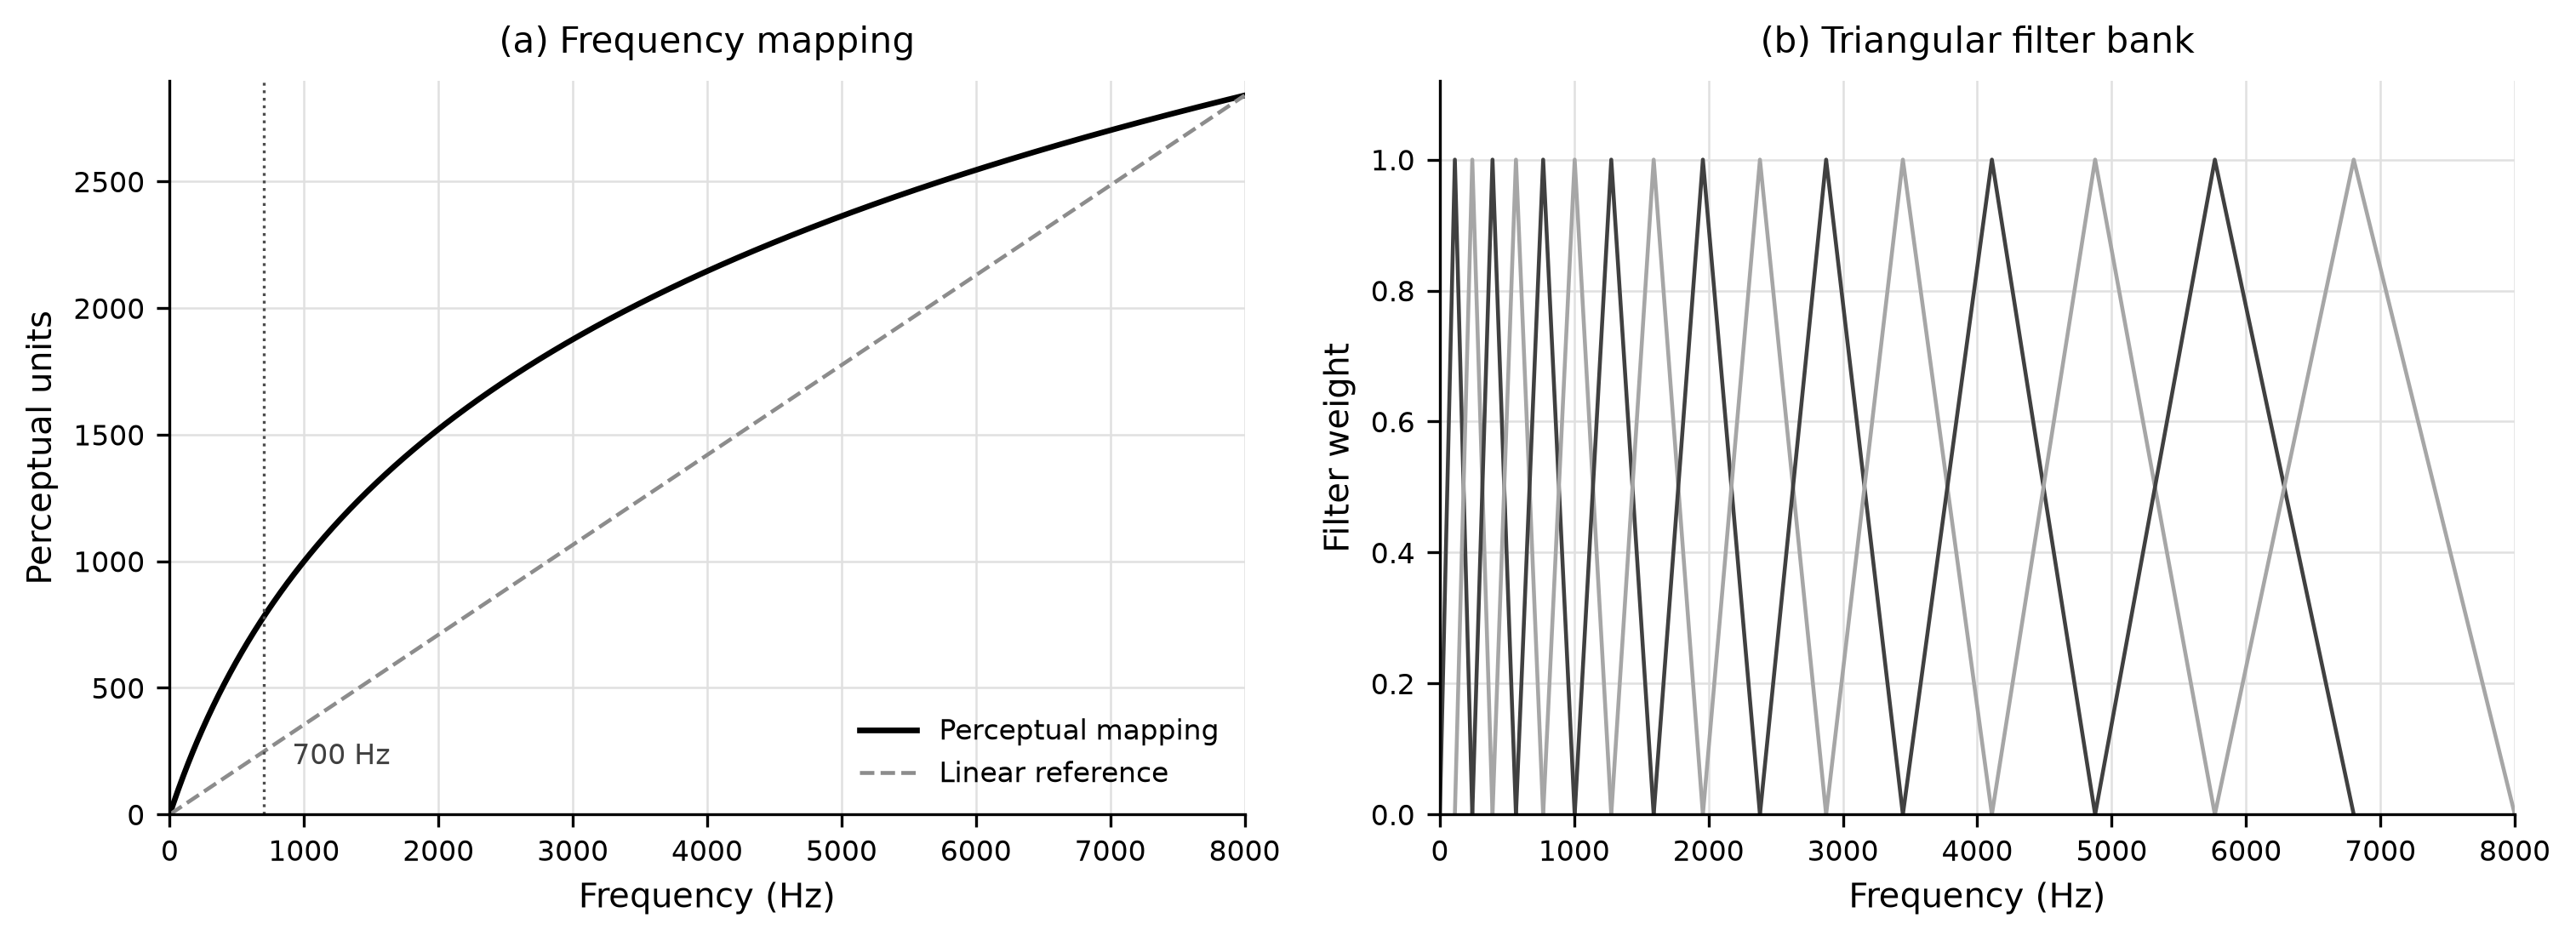
\includegraphics[width=\textwidth]{mel_mapping.png}
\caption{The perceptual frequency mapping of Equation~\eqref{eq:mel} in panel
(a), plotted against a linear reference over the band retained after
resampling, and in panel (b) a reduced bank of sixteen triangular filters
spaced uniformly on the warped axis and drawn against hertz. Beyond restating
the mapping, the figure shows what it costs and buys: filters near the bottom
of the band span on the order of 240~Hz while those near the top span on the
order of 2200~Hz, so fine structure above 4~kHz is deliberately pooled away
in exchange for resolution below 1~kHz. The bank used in the experiments has
128 filters rather than the sixteen drawn here, which are reduced in number
only so the individual triangles remain distinguishable.}
\label{fig:mel}
\end{figure}

The triangular weightings overlap, each beginning at the centre of the one
before it and ending at the centre of the one after, so that every frequency
contributes to exactly two filters and the resulting representation is smooth
in the filter index. Because the filters are uniformly spaced on the warped
axis, they become progressively wider in hertz as frequency rises, which is
what performs the compression: a filter near 4~kHz pools energy over a band
several times wider than one near 300~Hz, and the fine structure within the
wider band is deliberately discarded. The logarithmic amplitude scaling
applied afterwards compresses the dynamic range so that the low energy
portions of a recording, including the decaying tail of a cough, remain
visible alongside the high energy onset rather than being driven to the floor
of the image.

We use a Hamming window of 512 samples with 256 samples of overlap, a
transform length of 512 and 128 filters, and resize the resulting image to
$224 \times 224$ pixels to match the input expected by the transferred
architectures. At 16~kHz a 512 sample window spans 32~ms and advances by
16~ms, which is short enough to resolve the onset of a cough as a distinct
event and long enough to give usable frequency resolution. The resize is
performed after the logarithmic scaling rather than before, so that
interpolation acts on a quantity whose dynamic range has already been
compressed.

\subsection{Classification architectures}\label{sec:d-arch}

Four architectures are evaluated. One is trained from random initialisation
and three are transferred from a large image corpus with the classification
head replaced by a two unit layer. Table~\ref{tab:arch} summarises the
properties that bear on the comparison.

\begin{table}[t]
\centering
\footnotesize
\caption{The four architectures and the properties relevant to the
comparison. Depth is counted as weighted layers along the principal path. The
final column records the mechanism each architecture uses to propagate
information across depth, which is the property this study relates to the
benefit obtained from denoising.}
\label{tab:arch}
\begin{tabular}{@{}llll@{}}
\toprule
Architecture & Input & Initialisation & Propagation mechanism \\
\midrule
Compact network & Linear axis & Random & Plain stacked convolutions \\
ResNet18 & Perceptual axis & Transferred & Additive identity shortcuts \\
MobileNetV2 & Perceptual axis & Transferred & Inverted residual bottlenecks \\
DenseNet201 & Perceptual axis & Transferred & Concatenative dense reuse \\
\bottomrule
\end{tabular}
\end{table}

\subsubsection{Compact network trained from scratch}\label{sec:d-cnn}

The baseline comprises three convolutional layers, each followed by a pooling
operation that halves the spatial dimensions, and two fully connected layers
ending in a two unit output. It is trained from random initialisation on the
linear axis spectrograms and establishes what is achievable without
transferred weights. Its role is to separate two effects that are otherwise
confounded: the gain from the perceptual frequency axis and the gain from
transferred initialisation. Because this model differs from the others in both
respects, it is treated throughout as a reference point rather than as a
competitor, and the comparisons that carry the argument of the paper are made
among the three transferred models.

\subsubsection{Residual network}\label{sec:d-resnet}

ResNet18 introduces additive shortcut connections that carry the input of a
block forward to its output, so that each block learns a residual correction
rather than a complete transformation~\cite{he2016}. The arrangement allows
gradients to reach early layers without attenuation through the intervening
nonlinearities, which is what permits depth to be increased without the
degradation that plagued plain stacks. At eighteen weighted layers it is the
shallowest of the three transferred models, and its capacity is moderate by
current standards, which is the property that makes it informative here.

\subsubsection{Inverted residual network}\label{sec:d-mobilenet}

MobileNetV2 is designed for deployment under tight memory and power budgets.
It replaces standard convolutions with depthwise separable ones, factorising a
convolution into a spatial filtering step applied per channel and a pointwise
combination across channels, which reduces the parameter count and the
arithmetic by roughly an order of magnitude for a given receptive field. Its
blocks expand the channel dimension internally and project back to a narrow
linear bottleneck, with the shortcut connecting the bottlenecks rather than the
expanded representations~\cite{sandler2018}. Including it tests whether a
detector of practical size on portable hardware can approach the accuracy of a
larger model, which matters because a cough detector is most useful where it
can run continuously.

\subsubsection{Densely connected network}\label{sec:d-densenet}

DenseNet201 connects every layer within a block to all preceding layers by
concatenation rather than addition, so a layer has direct access to every
feature map produced before it~\cite{huang2017}. The arrangement strengthens
gradient flow and reduces redundancy, since a feature computed once need not
be recomputed downstream. It is by a wide margin the deepest of the models
considered. Its inclusion is deliberate rather than incidental: if the benefit
of denoising diminishes as a network becomes better able to form
representations that ignore interference, then the architecture with the most
extensive feature reuse is where that diminution should be visible, and
Section~\ref{sec:res-denoise} reports what is observed.

\subsection{Rationale for the architecture set}\label{sec:d-why}

The four models were not selected for coverage of the literature but to span
the mechanisms by which a network can achieve robustness to interference. The
compact network has no such mechanism beyond pooling. ResNet18 propagates
information additively through a moderate depth. MobileNetV2 is explicitly
constrained in capacity, so whatever robustness it attains must come from
structure rather than from parameters. DenseNet201 maximises feature reuse.
If denoising substitutes for architectural robustness, as
Section~\ref{sec:rel-denoise} argues it should, then its benefit ought to
decline along this ordering, and the set is arranged so that the prediction
can be tested.

\subsection{Computational considerations}\label{sec:d-cost}

The pipeline is intended for a setting in which audio arrives continuously, so
the cost of each stage is worth stating, both because it bounds what can run
on portable hardware and because it determines whether the optional denoising
stage is worth its place.

Conditioning is linear in the number of samples. For a recording of duration
$T$ seconds the resampling operation touches $T f_s$ samples once, and the
channel reduction is a single pass over the same data. The wavelet
decomposition of Equation~\eqref{eq:mra} is likewise linear: a fast wavelet
transform to level $J$ performs filtering and downsampling at each level, and
because each level operates on half the samples of the one before, the total
work is bounded by
\begin{equation}
\sum_{j=0}^{J-1} c \cdot \frac{T f_s}{2^{j}} < 2 c \, T f_s,
\label{eq:cost-dwt}
\end{equation}
where $c$ is the cost per sample of the filter pair. The decomposition
therefore costs less than twice a single filtering pass regardless of $J$,
which is why increasing the decomposition level is inexpensive and why the
choice of $J$ was governed by the band structure of the signal rather than by
cost. Thresholding and reconstruction are of the same order.

Spectrogram extraction is dominated by the transforms. With a window of
$L$ samples advancing by $L/2$, a recording yields approximately
$2 T f_s / L$ frames, each requiring a transform of cost
$\mathcal{O}(L \log L)$, so the total is $\mathcal{O}(T f_s \log L)$. The
perceptual representation adds the filter bank, which applies $M$ triangular
weightings to each frame at a cost proportional to $M L / 2$ per frame, and
the subsequent resize to the network input size. These are small relative to
the transforms themselves.

Inference dominates everything preceding it. A forward pass through a
transferred architecture on a $224 \times 224$ input requires on the order of
$10^8$ to $10^9$ multiply accumulate operations depending on the model, which
exceeds the cost of the entire preprocessing chain for a recording of a few
seconds by two or more orders of magnitude. Two consequences follow. The
first is that the denoising stage should be judged on whether it improves the
result rather than on its cost, which is negligible in comparison. The second
is that the choice of architecture is the decision that determines whether the
system can run continuously, which is the reason a capacity constrained model
is included in the comparison at all and why its result is reported alongside
the most accurate one in Section~\ref{sec:res-deploy} rather than being
treated as an also ran.

\section{Experimental setup}\label{sec:setup}

This section gives the corpus and its partition, the training configuration,
the metrics, and the information required to repeat the experiments.
Section~\ref{sec:s-data} describes the data, Section~\ref{sec:s-train} the
optimisation, Section~\ref{sec:s-metrics} the measures reported, and
Section~\ref{sec:s-repro} the reproducibility details.

\subsection{Corpus and partition}\label{sec:s-data}

Experiments use COUGHVID, an open corpus of crowdsourced recordings collected
through a web interface~\cite{orlandic2021}. Contributors submitted audio from
their own devices in their own surroundings, with no control over microphone
quality, distance, background noise or recording level, and a substantial
fraction of submissions contain no cough. That heterogeneity is the reason the
corpus is appropriate for the present question: a detector evaluated on
studio material would not be tested against the conditions that make
denoising worth considering.

All recordings were converted to WAV and assigned to one of two classes,
cough or noncough, and partitioned into training and test sets.
Table~\ref{tab:split} gives the composition. The partition is fixed across all
eight configurations, so every model is trained on the same recordings and
measured on the same held out material, and differences between configurations
cannot be attributed to a favourable split.

\begin{table}[t]
\centering
\footnotesize
\caption{Composition of the partition, identical for all eight
configurations. The imbalance of roughly 2.15 to 1 in favour of cough is a
property of the collection rather than of the partition, and
Section~\ref{sec:res-errors} shows that it inflates accuracy relative to
measures that weight the classes equally.}
\label{tab:split}
\begin{tabular}{@{}lrrr@{}}
\toprule
Partition & Cough & Noncough & Total \\
\midrule
Training & 12{,}495 & 5{,}808 & 18{,}303 \\
Test & 3{,}124 & 1{,}453 & 4{,}577 \\
\midrule
Total & 15{,}619 & 7{,}261 & 22{,}880 \\
\bottomrule
\end{tabular}
\end{table}

The imbalance deserves comment because it conditions how the results in
Section~\ref{sec:results} should be read. Coughs outnumber noncoughs by
slightly more than two to one in both partitions, which reflects the fact that
contributors to the corpus were asked to cough. A classifier that labelled
every test recording as cough would therefore be correct on 3,124 of 4,577
occasions, an accuracy of 68.26 percent, without having learned anything at
all. Every accuracy figure reported below should be read against that
reference rather than against 50 percent.

\subsection{Training configuration}\label{sec:s-train}

All models were trained in MATLAB using the Deep Learning Toolbox on a
workstation with an NVIDIA RTX 4050 graphics processor. Optimisation used
Adam with a batch size of 32 throughout, a learning rate of $10^{-3}$ for
every model except DenseNet201, and $10^{-4}$ for DenseNet201.
Table~\ref{tab:train} records the settings, including the three points on
which the configurations are not uniform.

\begin{table}[t]
\centering
\footnotesize
\caption{Training configuration. The epoch budget and the learning rate are
the two respects in which the transferred models were not treated
identically, and the material held out for measurement was also the material
monitored during training. Section~\ref{sec:res-limits} states what each of
these costs the interpretation of the results.}
\label{tab:train}
\begin{tabular}{@{}ll@{}}
\toprule
Setting & Value \\
\midrule
Framework & MATLAB Deep Learning Toolbox \\
Hardware & NVIDIA RTX 4050 \\
Optimiser & Adam \\
Learning rate, all models except DenseNet201 & $10^{-3}$ \\
Learning rate, DenseNet201 & $10^{-4}$ \\
Batch size & 32 \\
Epochs, compact network, ResNet18, MobileNetV2 & 10 \\
Epochs, DenseNet201 & 3 \\
Monitoring interval & every 50 iterations (ResNet18, MobileNetV2) \\
 & every 200 iterations (DenseNet201) \\
Data used for monitoring & the test partition \\
Network retained & the one at the final iteration \\
Random seed & not fixed \\
Sampling rate, perceptual axis models & 16~kHz, mono \\
Sampling rate, compact network & as recorded, mono \\
Wavelet & sym4, level 6, empirical Bayes \\
Linear axis spectrogram & 256 point window, 200 overlap, \\
 & 256 point transform \\
Perceptual spectrogram & 512 point window, 256 overlap, 128 filters \\
Network input size & $224 \times 224$ \\
\bottomrule
\end{tabular}
\end{table}

DenseNet201 was trained for three epochs against ten for the other two
transferred models, because its depth makes each epoch considerably more
expensive, and at a learning rate an order of magnitude lower. These are real
asymmetries in the experimental design and we do not present them as anything
else. Their consequence is discussed in Section~\ref{sec:res-limits}, where we
set out which of our conclusions they can and cannot affect.

Two further properties of the procedure must be stated plainly, because they
bear on how every number in Section~\ref{sec:results} should be read. The
first is that no separate validation partition was constructed. The test
partition was supplied to the training routine as the data against which
progress was monitored, and the accuracy reported for each configuration is
measured on that same material. No quantity computed on the test partition
was used to select weights, since the network retained is the one at the final
iteration rather than the one at the best monitored score, but the
arrangement removes the separation between the data used to observe training
and the data used to report performance. The figures below are therefore not
estimates of performance on unseen material in the strict sense, and we treat
them as measurements on a partition that was visible throughout rather than as
generalisation estimates.

The second is that the compact network and the three transferred networks do
not receive comparable inputs, and the difference is larger than the change of
frequency axis alone. For the transferred models the perceptual spectrogram is
computed as a matrix, compressed logarithmically, mapped to the unit interval
and written as a single channel image, which is then replicated across three
channels at load time. For the compact network the linear axis spectrogram is
drawn to a figure and the rendered figure is captured as a raster image, so
the network receives a picture of a plot rather than the transform itself,
carrying the display colour map and whatever resolution the rendering surface
provided. The two paths also differ in sample rate, because the recordings are
resampled to 16~kHz only on the perceptual axis branch. The comparison between
the compact network and the transferred networks therefore varies five things
at once, and Section~\ref{sec:res-limits} explains why we decline to attribute
the difference between them to any one of the five.

\subsection{Evaluation metrics}\label{sec:s-metrics}

Let TP and TN denote correctly classified cough and noncough recordings, and
FP and FN the two error types, where a false positive is a noncough recording
labelled as a cough. The primary measures are
\begin{align}
\text{Accuracy} &= \frac{\mathrm{TP} + \mathrm{TN}}
{\mathrm{TP} + \mathrm{TN} + \mathrm{FP} + \mathrm{FN}}, \label{eq:acc} \\[4pt]
\text{Precision} &= \frac{\mathrm{TP}}{\mathrm{TP} + \mathrm{FP}},
\label{eq:prec} \\[4pt]
\text{Recall} &= \frac{\mathrm{TP}}{\mathrm{TP} + \mathrm{FN}},
\label{eq:rec} \\[4pt]
F_1 &= \frac{2 \cdot \text{Precision} \cdot \text{Recall}}
{\text{Precision} + \text{Recall}}. \label{eq:f1}
\end{align}

Precision and recall are reported alongside accuracy because the two error
types carry unequal cost in this application. A false negative is a cough that
goes unrecorded, which in a monitored period may be recovered when the person
coughs again. A false positive admits audio containing no cough into a
downstream analysis that was not trained on such material, and the resulting
output is reported with a confidence value it has not earned. Precision is
therefore the quantity a screening deployment watches most closely, and
Section~\ref{sec:res-errors} examines how it is composed for the leading
configuration.

Because the partition is imbalanced, accuracy alone would be a misleading
summary, and all four measures are reported for every configuration so that a
gain arising from a shift toward the majority class can be distinguished from
a genuine improvement. The relationship between the four rates and the
underlying counts is set out in Appendix~\ref{app:derivation}.

\subsection{Reproducibility}\label{sec:s-repro}

A single run consists of the following steps, performed end to end for one
configuration. Every recording in the corpus is read, reduced to mono and
resampled to 16~kHz. Where the configuration calls for it, the waveform is
denoised by a level six sym4 decomposition with soft thresholding and
reconstructed. The conditioned waveform is converted to the spectrogram
representation the configuration specifies and, for the transferred models,
resized to $224 \times 224$. The classifier is initialised, either randomly or
from transferred weights with a replaced two unit head, and optimised with the
settings of Table~\ref{tab:train} over the 18,303 training recordings. The
trained model is then applied once to the 4,577 test recordings and the
confusion counts recorded, from which the rates reported in
Table~\ref{tab:main} are computed.

The experimental grid is the full cross of two factors over four
architectures, with the constraint that the compact network is paired only
with the linear axis representation and the transferred models only with the
perceptual one. This yields eight runs: the compact network with and without
denoising, and each of ResNet18, MobileNetV2 and DenseNet201 with and without
denoising. Each run is trained once, so the figures reported carry no estimate
of variation across random initialisations, a limitation addressed in
Section~\ref{sec:res-limits}.

Two secondary analyses are reported alongside the primary results. The first
takes the difference between the paired runs of each architecture, answering
the question of whether denoising acts in the same direction and by the same
mechanism across the four models rather than merely whether it raises
accuracy; its result appears in Table~\ref{tab:delta}. The second examines
the confusion counts of the two ResNet18 configurations, answering the
question of how the improvement attributed to denoising is distributed
between the two error types; its result appears in Table~\ref{tab:resnet}.
Both use quantities recorded during the
evaluation runs described above and require no additional training. The
arithmetic relating the counts to the summary rates is given in
Appendix~\ref{app:derivation}, so that every figure in the body can be
checked against every other.

\section{Results and discussion}\label{sec:results}

This section reports the outcome of the eight configurations and interprets
them. Section~\ref{sec:res-overall} gives the headline comparison.
Section~\ref{sec:res-axis} isolates the contribution of the frequency axis,
and Section~\ref{sec:res-denoise} that of wavelet denoising.
Section~\ref{sec:res-errors} examines the error structure of the leading
architecture in detail. Section~\ref{sec:res-deploy} considers what the
figures imply for a deployed system, and Section~\ref{sec:res-limits} states
the limits of the study.

\subsection{Overall comparison}\label{sec:res-overall}

Table~\ref{tab:main} reports accuracy, precision, recall and $F_1$ for every
configuration on the held out partition. The highest accuracy, 96.53 percent,
is obtained by ResNet18 operating on denoised perceptual spectrograms, with a
precision of 97.59 percent, a recall of 97.31 percent and an $F_1$ of 97.45
percent. This represents a cumulative improvement of 3.08 accuracy points over
the compact network on linear axis spectrograms, which is the configuration
that uses neither transferred weights, nor perceptual scaling, nor denoising.

\begin{table}[t]
\centering
\footnotesize
\caption{Performance of all eight configurations on the 4,577 held out
recordings. The compact network is trained from random initialisation on the
linear frequency axis; the three transferred architectures operate on the
perceptual axis. Accuracy should be read against a majority class baseline of
68.26 percent rather than against 50 percent, because the test partition
contains 2.15 cough recordings for every noncough recording.}
\label{tab:main}
\begin{tabular}{@{}llrrrr@{}}
\toprule
Architecture & Input representation & Accuracy (\%) & Precision & Recall & $F_1$ \\
\midrule
Compact network & Linear & 93.45 & 0.9754 & 0.9273 & 0.9508 \\
Compact network & Wavelet + linear & 93.86 & 0.9665 & 0.9427 & 0.9545 \\
ResNet18 & Perceptual & 95.76 & 0.9584 & 0.9805 & 0.9693 \\
ResNet18 & Wavelet + perceptual & \textbf{96.53} & \textbf{0.9759} & 0.9731 & \textbf{0.9745} \\
MobileNetV2 & Perceptual & 95.76 & 0.9797 & 0.9577 & 0.9686 \\
MobileNetV2 & Wavelet + perceptual & 96.11 & 0.9700 & 0.9731 & 0.9716 \\
DenseNet201 & Perceptual & 96.15 & 0.9694 & 0.9744 & 0.9719 \\
DenseNet201 & Wavelet + perceptual & 96.09 & 0.9652 & 0.9779 & 0.9715 \\
\bottomrule
\end{tabular}
\end{table}

Two features of the table deserve comment before the individual factors are
separated. The first is that the three transferred architectures lie close
together, spanning 0.77 accuracy points across their six configurations, while
the gap between the best transferred configuration and the compact network is
2.67 points. That gap is the only difference in the table wide enough to
exceed the uncertainty attaching to a single accuracy measurement, for the
reasons set out in Section~\ref{sec:res-precision}, and it is correspondingly
the only one on which a claim could rest. It will not carry the claim that
transferred initialisation is what produced it. The compact network differs
from the transferred networks in five respects simultaneously: the
initialisation, the architecture, the frequency axis, the sample rate at which
the recording was analysed, and whether the network is presented with the
spectrogram as a numerical array or with a raster image of that spectrogram as
plotted to a figure. Any one of the five is capable of moving accuracy by more
than two points, and the design separates none of them. We therefore report
the gap and decline to attribute it. The second feature is that every
configuration exceeds the majority class baseline of 68.26 percent by at least
25 points, so all eight models have learned structure in the signal rather
than exploiting the prior.

Figure~\ref{fig:results} presents the same eight configurations graphically,
paired so that the two bars above each architecture differ only in whether
denoising was applied. Reading across the four pairs shows that the gap
between architectures is wider than the gap produced by denoising within any
one of them, and reading within each pair shows that the sign of the
denoising effect is not constant across architectures, which is the
observation Section~\ref{sec:res-denoise} develops.

\begin{figure}[t]
\centering
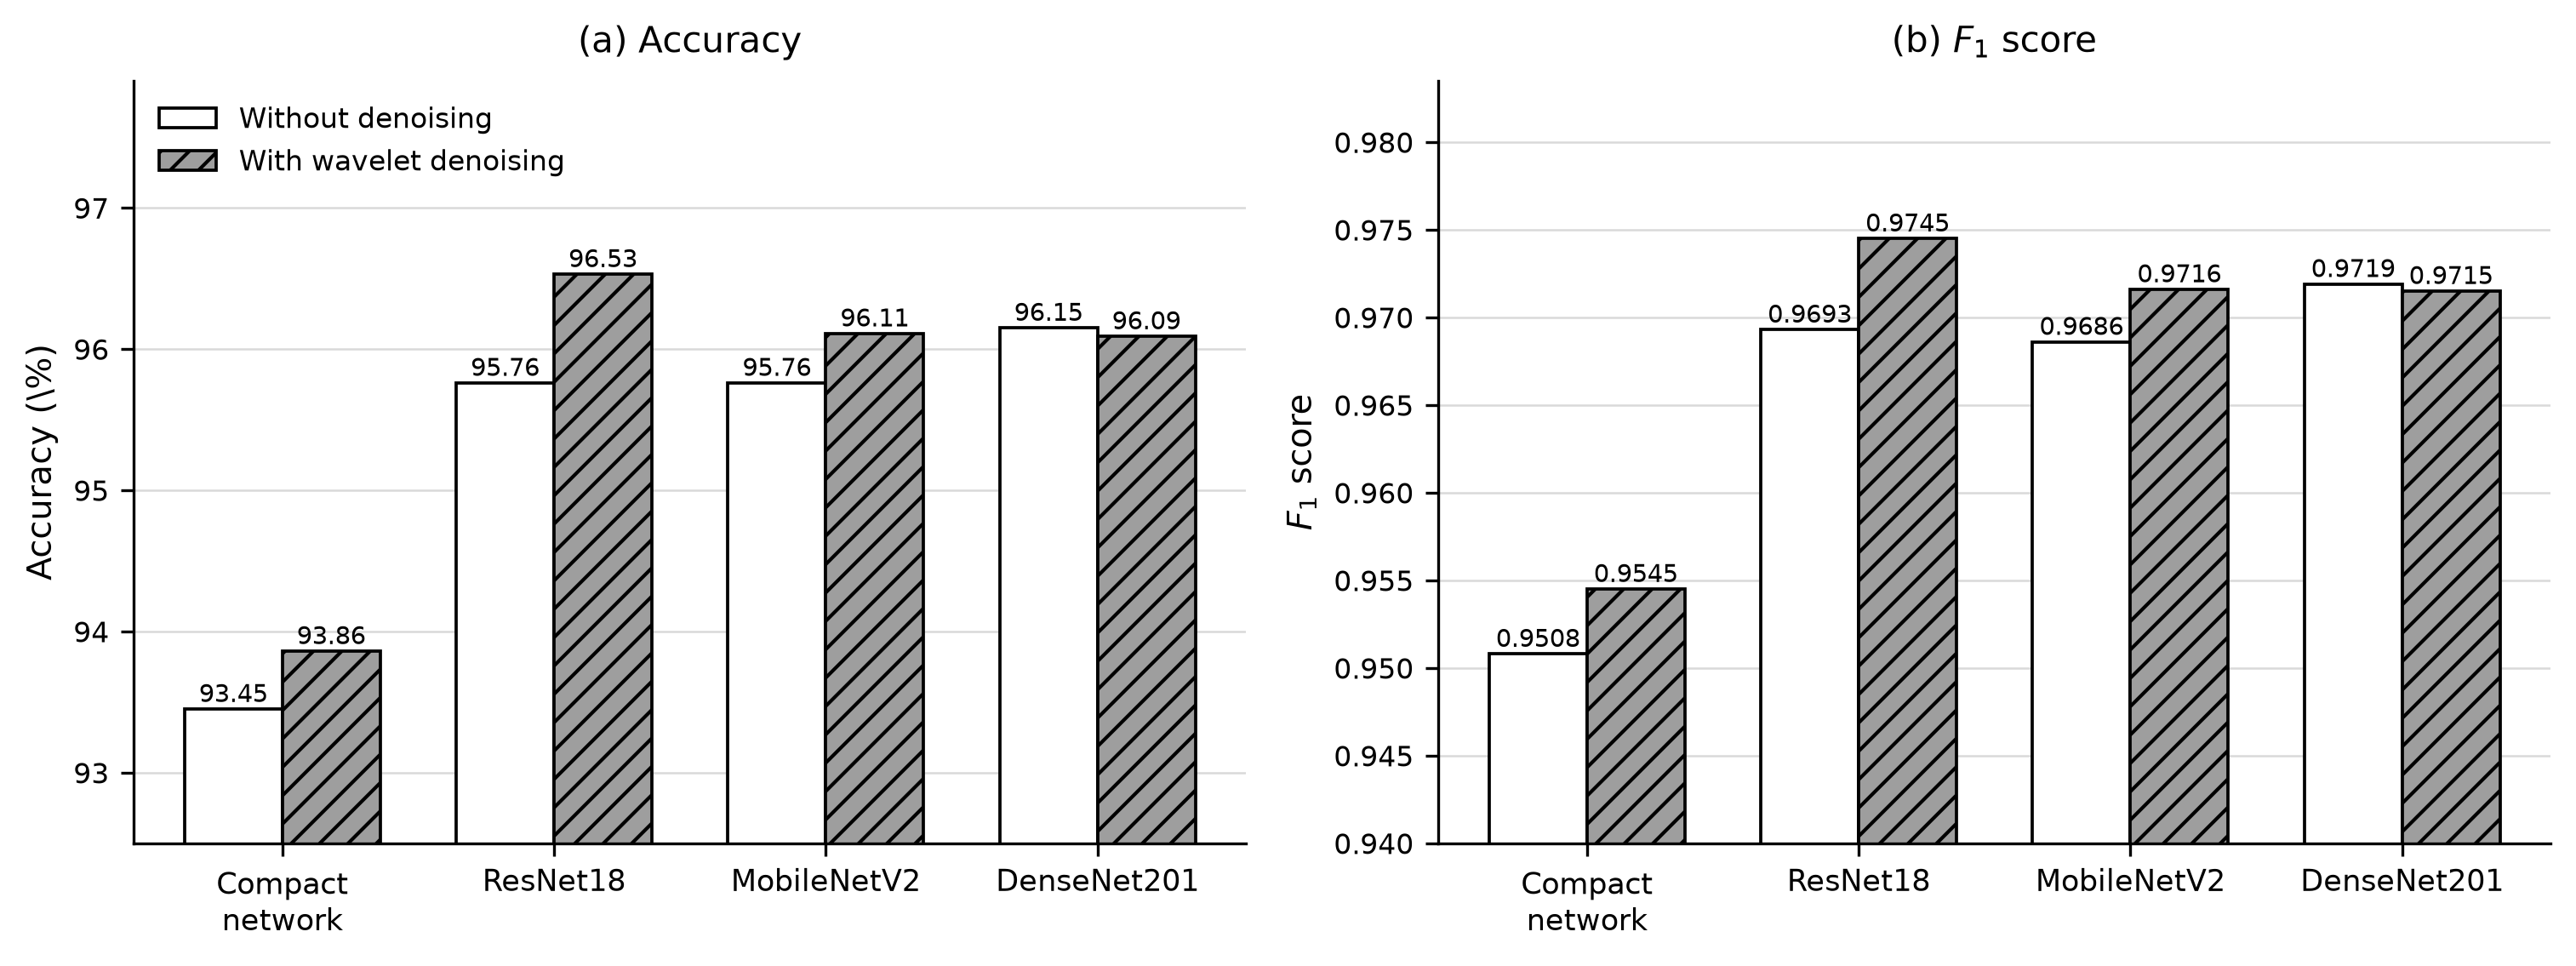
\includegraphics[width=\textwidth]{results_comparison.png}
\caption{Accuracy in panel (a) and $F_1$ score in panel (b) for the four
architectures, with the unfilled bar of each pair giving the result without
denoising and the hatched bar the result with it. The vertical axes are
truncated so that differences of a few tenths of a point remain visible;
every bar shown lies far above the majority class baseline of 68.26 percent.
Beyond the values already listed in Table~\ref{tab:main}, the paired layout
makes the inconsistency of the denoising effect apparent at a glance: three
pairs step upward and the fourth does not.}
\label{fig:results}
\end{figure}

\subsection{Effect of the frequency axis}\label{sec:res-axis}

Replacing the linear frequency axis with a perceptual one produced a
consistent improvement. The compact network on linear axis spectrograms
reached 93.45 percent, while ResNet18 on perceptual spectrograms reached 95.76
percent, a gain of 2.31 points, and every configuration using the perceptual
axis outperformed every configuration using the linear one without exception
across the eight runs.

The mechanism is a matter of where spectral resolution is spent. A linear axis
allocates bins uniformly, so half of them describe the band above 4~kHz, in
which a cough and many competing impulsive sounds are broadly similar. The
mapping of Equation~\eqref{eq:mel} compresses that band and expands the region
below roughly 1~kHz, where the voiced termination of a cough and much of the
envelope structure that separates it from a brief mechanical noise both
reside. Because a convolutional kernel is spatially uniform, it treats equal
distances along the frequency axis as equivalent regardless of what those
distances represent, so warping the axis changes what a kernel of a given size
is able to express. This is the argument originally advanced for perceptual
scaling in speech recognition~\cite{davis1980}, and the present results
indicate that it carries over to respiratory sounds.

The comparison is not a clean isolation of the representation, because the
compact network differs from the transferred models in initialisation and
depth as well as in input. The figure therefore bounds the combined effect
rather than attributing it, and Section~\ref{sec:res-limits} returns to this.

\subsection{Effect of wavelet denoising}\label{sec:res-denoise}

Wavelet preprocessing improved accuracy for three of the four architectures.
The gain was largest for ResNet18, which rose from 95.76 to 96.53 percent, an
improvement of 0.77 points. Its precision rose from 0.9584 to 0.9759 and its
$F_1$ from 0.9693 to 0.9745, indicating that the improvement came principally
from a reduction in false alarms rather than from detecting additional coughs.
MobileNetV2 improved from 95.76 to 96.11 percent, a gain of 0.35 points,
showing that an architecture constrained in capacity also benefits from a
cleaner input. The compact network improved from 93.45 to 93.86 percent.
These outcomes are consistent with the established view that attenuating
interference in a wavelet basis raises the effective signal to noise ratio of
a recording before any time frequency representation is
formed~\cite{mallat1989, donoho1995}.

DenseNet201 was the exception. Its accuracy changed from 96.15 to 96.09
percent, a difference of 0.06 points in the opposite direction and smaller
than the rounding in the reported figures. Recall improved slightly, from
0.9744 to 0.9779, while precision fell from 0.9694 to 0.9652, leaving $F_1$
essentially unchanged at 0.9719 against 0.9715. The most plausible reading is
that dense connectivity already supplies what denoising would otherwise
provide. Because every layer in a dense block receives the feature maps of all
preceding layers, the network has direct access to representations at many
levels of abstraction simultaneously and can learn to discount interference
without that interference being removed beforehand~\cite{huang2017}. On this
account denoising and dense connectivity are substitutes rather than
complements, and applying both yields little beyond applying either. There is
a further possibility that the two cannot be separated here: removing
components in a wavelet basis also removes some genuine high frequency
transient energy, and a network that had learned to exploit that energy would
lose a little by its removal.

Table~\ref{tab:delta} collects the change each architecture shows when
denoising is applied, so that the four comparisons can be read against one
another rather than recovered from eight separate rows. The accuracy column
orders the architectures by how much they gain, and the precision and recall
columns show that the gain is not of the same kind in each case: for ResNet18
precision rises while recall falls, whereas for the compact network and
MobileNetV2 the movement is in the opposite direction.

\begin{table}[t]
\centering
\footnotesize
\caption{Change in each measure when wavelet denoising is applied, by
architecture, computed from the paired rows of Table~\ref{tab:main}. Accuracy
is in percentage points and the remaining columns in absolute units. A
positive entry indicates that denoising improved the measure.}
\label{tab:delta}
\begin{tabular}{@{}lrrrr@{}}
\toprule
Architecture & $\Delta$ Accuracy & $\Delta$ Precision & $\Delta$ Recall & $\Delta F_1$ \\
\midrule
ResNet18 & $+0.77$ & $+0.0175$ & $-0.0074$ & $+0.0052$ \\
Compact network & $+0.41$ & $-0.0089$ & $+0.0154$ & $+0.0037$ \\
MobileNetV2 & $+0.35$ & $-0.0097$ & $+0.0154$ & $+0.0030$ \\
DenseNet201 & $-0.06$ & $-0.0042$ & $+0.0035$ & $-0.0004$ \\
\bottomrule
\end{tabular}
\end{table}

The practical implication is that wavelet denoising is most worthwhile for
architectures of moderate depth and capacity, and least worthwhile for very
deep networks with strong feature reuse. This is a useful result for system
design, because it indicates that preprocessing and architectural capacity
should be chosen together rather than independently.

\subsection{Error structure of the leading configuration}\label{sec:res-errors}

The accuracy figures summarise performance but conceal how the two error types
are distributed, which matters because the two carry different costs in a
screening context. Table~\ref{tab:resnet} gives the confusion counts for the
two ResNet18 configurations.

\begin{table}[t]
\centering
\footnotesize
\caption{Confusion counts for the two ResNet18 configurations on the 4,577
held out recordings. Where Table~\ref{tab:main} reports the summary rates,
this table shows how each rate is composed, which is what reveals that the
improvement from denoising is concentrated almost entirely in the false
positive column.}
\label{tab:resnet}
\begin{tabular}{@{}lrrrr@{}}
\toprule
Configuration & True positives & False negatives & False positives & True negatives \\
\midrule
Perceptual axis & 3063 & 61 & 133 & 1320 \\
Wavelet + perceptual axis & 3040 & 84 & \textbf{75} & \textbf{1378} \\
\bottomrule
\end{tabular}
\end{table}

Figure~\ref{fig:confusion} presents the same two results as class by class
matrices. Where Table~\ref{tab:resnet} gives the four counts for arithmetic
use, the matrices show at a glance that the entire difference between the two
configurations sits in the lower left cell, with the diagonal and the upper
right cell changing comparatively little.

\begin{figure}[t]
\centering
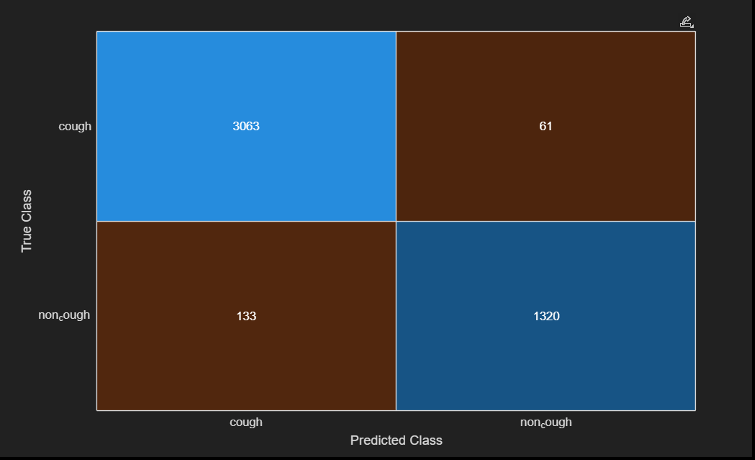
\includegraphics[width=0.72\textwidth]{cm_baseline.png}\\[6pt]
{\footnotesize (a) perceptual axis, without denoising}\\[10pt]
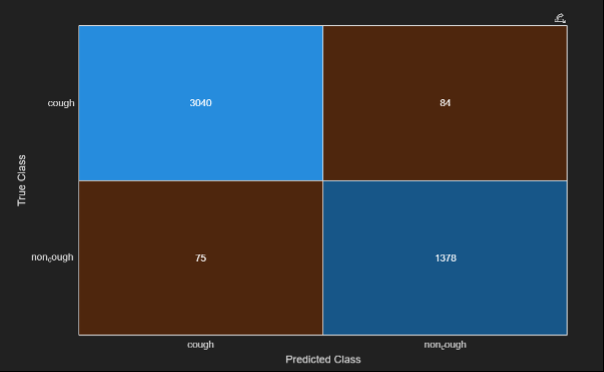
\includegraphics[width=0.72\textwidth]{cm_denoised.png}\\[6pt]
{\footnotesize (b) perceptual axis, with wavelet denoising}
\caption{Class by class results for the two ResNet18 configurations, with
true class on the vertical axis and predicted class on the horizontal. The
noncough row is the one that changes: 133 noncough recordings are labelled
as coughs in (a) against 75 in (b), while the cough row moves by 23 in the
opposite direction. The visual form makes the asymmetry of the change
apparent in a way the four numbers alone do not, since the off diagonal mass
is concentrated almost entirely in a single cell in both panels.}
\label{fig:confusion}
\end{figure}

Without denoising, the model identified 3,063 of the 3,124 cough recordings,
giving a recall of 0.9805, so almost every genuine cough was found. The cost
was 133 noncough recordings classified as coughs, which produced the
comparatively low precision of 0.9584. With denoising, false positives fell
from 133 to 75, a reduction of 43.6 percent, and true negatives rose
correspondingly from 1,320 to 1,378. Recall fell slightly, to 0.9731, as false
negatives rose from 61 to 84. The net effect was an increase in $F_1$ from
0.9693 to 0.9745.

This redistribution is favourable for the intended application. A false
positive at the detection stage admits audio containing no cough into a
downstream analysis that was never trained on such material, and the output of
that analysis is then reported with a confidence value it has not earned. In a
screening deployment this generates referrals that consume clinical time and
erode trust in the system among those who must act on its output. Trading 23
additional missed coughs for 58 fewer false alarms is therefore a reasonable
exchange, particularly where the same person may cough more than once within a
monitored period and a missed event does not necessarily mean a missed case.

\subsection{Implications for deployment}\label{sec:res-deploy}

Three observations follow for a system intended to run outside a laboratory.

The first concerns the choice of architecture under a computational budget.
MobileNetV2 with denoising reached 96.11 percent, within 0.42 points of the
best configuration, while requiring a fraction of the parameters and
arithmetic of the larger models by virtue of its depthwise separable
convolutions and inverted residual blocks~\cite{sandler2018}. Where a detector
must run continuously on a handheld or embedded device, which is the setting
in which cough monitoring is most useful and where comparable systems have
been targeted~\cite{hoyosbarcelo2018, karatas2021}, this configuration is the
more sensible selection.

The second concerns whether to include the denoising stage at all. Its cost is
linear in recording length and it must be applied to every input, both in
training and at inference. For ResNet18 and MobileNetV2 the gain justifies
that cost. For DenseNet201 it does not, and the stage should be omitted,
which also removes a parameter choice, the wavelet family and decomposition
level, that would otherwise have to be validated for each new deployment.

The third concerns the operating point. All the figures reported here derive
from the default decision rule in which the more probable class is selected.
Because the two error types are not equally costly, a deployed system would
normally adjust the decision threshold to favour specificity, and the
consequence of doing so can be anticipated from Table~\ref{tab:resnet}: the
undenoised configuration has the headroom in recall to absorb such an
adjustment, whereas the denoised configuration is already operating closer to
a balanced point.

\subsection{Statistical precision}\label{sec:res-precision}

The differences discussed above are small, and their interpretation depends on
how precisely a proportion measured on 4,577 recordings is known. We therefore
attach an interval to every accuracy figure and report measures that do not
inherit the class imbalance. Each accuracy is a binomial proportion estimated
on a finite sample, and we summarise its precision with the Wilson score
interval, which is preferred to the normal approximation because it remains
inside the unit interval and keeps its nominal coverage when the proportion
approaches one, as all of these do~\cite{brown2001}. Because accuracy on a
corpus with 2.15 coughs for every noncough recording is dominated by the
majority class, we also report specificity, the proportion of noncough
recordings correctly rejected, together with balanced accuracy, the unweighted
mean of recall and specificity, and the Matthews correlation coefficient,
which uses all four cells of the confusion matrix and is the measure least
distorted by imbalance~\cite{chicco2020}. Table~\ref{tab:interval} collects
these for the eight configurations.

\begin{table}[t]
\centering
\footnotesize
\caption{Interval estimates and class balanced measures for the eight
configurations. Accuracy is accompanied by its 95 percent Wilson score
interval on the 4,577 test recordings. Specificity is the proportion of the
1,453 noncough recordings correctly rejected, balanced accuracy the unweighted
mean of recall and specificity, and MCC the Matthews correlation coefficient.
Wav abbreviates wavelet denoising applied before spectrogram extraction, and
Perc the perceptual frequency axis. The interval around every individual
accuracy is wider than any difference between a configuration and its pair.}
\label{tab:interval}
\begin{tabular}{@{}llrcrrr@{}}
\toprule
Architecture & Input & Acc. & 95\% interval & Spec. & Bal. & MCC \\
\midrule
Compact & Linear & 93.45 & 92.69--94.13 & 94.98 & 93.85 & 0.855 \\
Compact & Wav + linear & 93.86 & 93.13--94.52 & 92.98 & 93.63 & 0.861 \\
ResNet18 & Perc & 95.76 & 95.14--96.31 & 90.85 & 94.45 & 0.901 \\
ResNet18 & Wav + Perc & \textbf{96.53} & 95.96--97.02 & 94.84 & \textbf{96.07} & \textbf{0.920} \\
MobileNetV2 & Perc & 95.76 & 95.14--96.31 & \textbf{95.73} & 95.75 & 0.904 \\
MobileNetV2 & Wav + Perc & 96.11 & 95.51--96.63 & 93.53 & 95.42 & 0.910 \\
DenseNet201 & Perc & 96.15 & 95.56--96.67 & 93.39 & 95.42 & 0.911 \\
DenseNet201 & Wav + Perc & 96.09 & 95.49--96.61 & 92.43 & 95.11 & 0.909 \\
\bottomrule
\end{tabular}
\end{table}

The intervals settle the status of the denoising comparisons. Their mean width
is 1.20 accuracy points, while the largest difference denoising produces in
any pair is 0.77 points on ResNet18 and the smallest is 0.06 points on
DenseNet201. Every difference the study reports between a configuration and
its denoised counterpart is therefore smaller than the uncertainty on either
of the two measurements being compared, and the intervals of all four pairs
overlap substantially. On this evidence the effect of denoising on accuracy is
not resolved by the experiment in either direction: the data are consistent
with a small benefit, with no effect, and with a small cost, and the pattern
of signs across the four architectures carries no more information than the
magnitudes do. The same arithmetic applies to the 0.77 point spread across the
three transferred architectures, which is likewise contained within a single
interval and does not support ranking them.

It should be said precisely what would settle the question, because the
present design cannot. A paired comparison of two classifiers on identical
test material is properly tested by McNemar's statistic, which depends only on
the two discordant counts, the recordings one model classifies correctly and
the other does not~\cite{dietterich1998}. Those counts are properties of the
paired per recording decisions and are not recoverable from confusion
matrices, which report only the margins. The margins do bound the discordance
from below: between the two ResNet18 configurations at least 81 of the 4,577
recordings must be classified differently, since 58 false positives are
removed and 23 false negatives introduced. The sign and size of the effect,
however, require the decisions themselves, which means retaining per recording
predictions for every configuration. We note this as a requirement on the
design rather than as a result.

The class balanced measures also change which configuration appears best, and
in a way accuracy conceals. Specificity varies across the eight configurations
from 90.85 to 95.73 percent, a spread of 4.88 points that is four times the
width of an accuracy interval and the largest systematic variation anywhere in
the study. ResNet18 on undenoised perceptual spectrograms has the weakest
specificity in the table at 90.85 percent, yet its accuracy of 95.76 percent
is identical to that of MobileNetV2 on the same input, which rejects noncough
material at 95.73 percent. Two configurations indistinguishable on accuracy
thus differ by almost five points in the rate at which they raise false
alarms, which is the quantity that governs whether a continuously running
detector is tolerable to use. Balanced accuracy and the Matthews coefficient
both rank the denoised ResNet18 configuration first, at 96.07 percent and
0.920 respectively, and both separate the compact network from the transferred
ones by a margin larger than they separate the transferred ones from each
other. These two measures are the ones we would ask a reader to compare, and
the ranking they produce is the one the discussion above relies on.

\subsection{Limitations}\label{sec:res-limits}

Six limitations bound what the present results establish, and we state them
with their consequences rather than deferring them.

The training budget is not uniform across the transferred models. DenseNet201
was optimised for three epochs against ten for ResNet18 and MobileNetV2, as
recorded in Table~\ref{tab:train}, because its depth makes each epoch
substantially more expensive. The observation that denoising does not benefit
DenseNet201 is therefore consistent with two explanations, dense connectivity
substituting for preprocessing or simply a shorter optimisation, and the
present experiments cannot separate them. Training to a matched budget is the
direct way to settle this, and until that is done the architectural reading
should be treated as the more plausible of two accounts rather than as an
established result. The interaction between normalisation statistics and a
short schedule gives further reason for caution, since those statistics are
themselves still settling in the early epochs of
training~\cite{awais2021}.

Each configuration was trained once, and the random seed was not fixed, so
neither an estimate of variation across initialisations nor an exact
reproduction of any individual run is available. This is the most serious of
the six, because Section~\ref{sec:res-precision} shows that every difference
the study reports between a configuration and its denoised counterpart is
smaller than the sampling uncertainty on a single accuracy measurement, before
any variation between runs is added. The consequence is that the denoising
comparisons are unresolved rather than negative, and that the ordering of the
three transferred architectures is not established. Only two findings survive
this limitation: the 2.67 point separation between the compact network and the
transferred networks, which exceeds the interval width but is confounded five
ways and is therefore reported without attribution, and the 4.88 point spread
in specificity, which exceeds it by a wider margin. Repeating every
configuration across several seeds and reporting the distribution rather than
a single value is the minimum that would change this, and retaining per
recording predictions so that paired tests become available is what would
settle the denoising question.

The comparison between frequency axes is confounded with initialisation and
depth, as noted in Section~\ref{sec:res-axis}, because the linear axis was
paired only with the compact network. The consistency of the direction across
all eight runs supports the conclusion that the representation contributes,
but the portion of the 2.31 point gap attributable to the axis alone is not
identified by this design. Pairing a transferred architecture with linear axis
input would resolve it.

No separate validation partition was constructed. The material on which the
reported accuracies are measured is the same material that was supplied to the
training routine for monitoring, as recorded in Table~\ref{tab:train}. The
network retained in each case is the one at the final iteration rather than
the one at the best monitored score, so no quantity computed on the test
partition entered the selection of weights, and the figures are not inflated
by that mechanism. What the arrangement does remove is the separation between
the data used to observe training and the data used to report performance,
which means the numbers should be read as measurements on a partition that was
visible throughout rather than as estimates of performance on unseen
recordings. A three way division of the corpus, with the epoch budget and the
learning rate chosen on a validation partition and the test partition touched
once, is the correction, and it is a precondition for the other improvements
listed here rather than an alternative to them.

The inputs given to the compact network and to the transferred networks differ
in more than the frequency axis. The perceptual spectrograms are computed as
arrays, compressed logarithmically and written as single channel images,
whereas the linear axis spectrograms are produced by plotting each transform
to a figure and capturing the rendered figure as a raster image, so the
compact network is presented with a picture of a plot rather than with the
transform. The two paths also analyse the recordings at different sample
rates. The practical consequences are twofold. The gap between the compact
network and the transferred networks cannot be assigned to initialisation,
architecture, frequency axis, sample rate or input encoding, because all five
vary together, and the linear axis images cannot be regenerated exactly by
anyone, including us, because a figure capture depends on the resolution and
the colour handling of the surface it was rendered on. Recomputing the linear
axis spectrograms as arrays on the same 16~kHz material, and pairing them with
a transferred architecture, would remove the confound and restore
reproducibility at the same time; this is the single change we would make
first.

The evaluation is confined to one corpus and to the binary task. COUGHVID is
crowdsourced and acoustically heterogeneous, which makes it a demanding test,
but its recordings were contributed by people who had been asked to cough, so
the character of its noncough class may differ from the continuous ambient
audio a deployed detector would encounter~\cite{orlandic2021}. Nothing
established here demonstrates that the ranking transfers to clinical
recordings, to a different distribution of noncough material, or to the finer
grained problem of distinguishing cough types rather than detecting coughing,
and extending the evaluation across corpora and to multiclass respiratory
discrimination is the direction in which the work should be taken.

\section{Conclusion}\label{sec:conclusion}

We have examined three design choices for binary cough detection on
crowdsourced audio and shown that they interact in ways a single factor study
would not reveal: perceptual frequency scaling improved every architecture to
which it was applied, the separation between the compact network and the
transferred networks was wider than any separation among the transferred
networks themselves, and wavelet denoising before spectrogram extraction
produced differences that this design is not precise enough to resolve. The best
configuration, a residual network of moderate depth applied to denoised
perceptual spectrograms, reached 96.53 percent accuracy with a precision of
97.59 percent, a recall of 97.31 percent and an $F_1$ of 97.45 percent, a
cumulative gain of 3.08 accuracy points over a compact network trained from
scratch on linear axis spectrograms, and its advantage arose principally from
a 43.6 percent reduction in false alarms rather than from detecting additional
coughs. Denoising also benefited the capacity constrained network, which
reached 96.11 percent while remaining small enough for continuous operation on
portable hardware, but it did not benefit the densely connected network, whose
accuracy was unchanged within rounding, and we read this as evidence that
explicit preprocessing and architectural feature reuse address the same
problem by different means and are therefore substitutes rather than
complements; the practical consequence is that preprocessing and capacity
should be selected together rather than independently, with the residual
network and denoising preferred where accuracy is paramount and the capacity
constrained network preferred where the detector must run continuously under a
power budget.

\begin{appendices}

\section{Composition of the reported rates}\label{app:derivation}

The summary rates in Table~\ref{tab:main} and the counts in
Table~\ref{tab:resnet} are related by the definitions of
Section~\ref{sec:s-metrics}, and the relationship is set out here so that the
figures in the body can be checked against one another without recourse to the
original result files.

For a test partition containing $P$ cough and $N$ noncough recordings, the
four cells of the confusion matrix follow from recall and precision by
\begin{equation}
\mathrm{TP} = \mathrm{Recall} \cdot P, \qquad
\mathrm{FN} = P - \mathrm{TP},
\label{eq:app-tp}
\end{equation}
\begin{equation}
\mathrm{FP} = \mathrm{TP} \cdot
\frac{1 - \mathrm{Precision}}{\mathrm{Precision}}, \qquad
\mathrm{TN} = N - \mathrm{FP},
\label{eq:app-fp}
\end{equation}
where Equation~\eqref{eq:app-fp} follows from rearranging the definition of
precision in Equation~\eqref{eq:prec}. With $P = 3124$ and $N = 1453$ from
Table~\ref{tab:split}, the ResNet18 configuration without denoising has
$\mathrm{TP} = 0.9805 \times 3124 = 3063$ and
$\mathrm{FP} = 3063 \times 0.0416 / 0.9584 = 133$, which are the counts
recorded in Table~\ref{tab:resnet}.

Accuracy recovered from these counts is
\begin{equation}
\frac{\mathrm{TP} + \mathrm{TN}}{P + N}
= \frac{3063 + 1320}{4577} = 0.9576,
\label{eq:app-acc}
\end{equation}
in agreement with the 95.76 percent reported in Table~\ref{tab:main}. The
same arithmetic applied to the denoised configuration gives
$(3040 + 1378)/4577 = 0.9653$, matching the 96.53 percent reported there.

Two consequences of the class composition are worth stating explicitly. A
classifier assigning every recording to the majority class would achieve
$P/(P+N) = 0.6826$, which is the reference against which the accuracy column
should be read. And because $P$ exceeds $N$ by a factor of 2.15, a given
number of false positives depresses precision more than the same number of
false negatives depresses recall, which is why the reduction of 58 false
positives discussed in Section~\ref{sec:res-errors} moves precision by 1.75
points while the accompanying increase of 23 false negatives moves recall by
only 0.74 points.

\end{appendices}

\backmatter

\begin{thebibliography}{31}

\bibitem{brown2020}
Brown, C., Chauhan, J., Grammenos, A., et al.: Exploring automatic diagnosis
of COVID-19 from crowdsourced respiratory sound data. In: Proceedings of the
26th ACM SIGKDD International Conference on Knowledge Discovery and Data
Mining, pp. 3474--3484 (2020)

\bibitem{imran2020}
Imran, A., Posokhova, I., Qureshi, H.N., Masood, U., et al.: AI4COVID-19: AI
enabled preliminary diagnosis for COVID-19 from cough samples via an app.
Informatics in Medicine Unlocked \textbf{20}, 100378 (2020)

\bibitem{laguarta2020}
Laguarta, J., Hueto, F., Subirana, B.: COVID-19 artificial intelligence
diagnosis using only cough recordings. IEEE Open Journal of Engineering in
Medicine and Biology \textbf{1}, 275--281 (2020)

\bibitem{orlandic2021}
Orlandic, L., Teijeiro, T., Atienza, D.: The COUGHVID crowdsourcing dataset, a
corpus for the study of large-scale cough analysis algorithms. Scientific Data
\textbf{8}(1) (2021)

\bibitem{swarnkar2013}
Swarnkar, V., Abeyratne, U.R., Chang, A.B., Amrulloh, Y.A., et al.: Automatic
identification of wet and dry cough in pediatric patients with respiratory
diseases. Annals of Biomedical Engineering \textbf{41}(5), 1016--1028 (2013)

\bibitem{hoyosbarcelo2018}
Hoyos-Barcel\'o, C., Monge-\'Alvarez, J., Shakir, M.Z., et al.: Efficient
$k$-NN implementation for real-time detection of cough events in smartphones.
IEEE Journal of Biomedical and Health Informatics \textbf{22}(5), 1662--1671
(2018)

\bibitem{mongealvarez2019}
Monge-\'Alvarez, J., Hoyos-Barcel\'o, C., Lesso, P., Casaseca-de-la-Higuera,
P.: Robust detection of audio-cough events using local Hu moments. IEEE
Journal of Biomedical and Health Informatics \textbf{23}(1), 184--196 (2019)

\bibitem{piczak2015}
Piczak, K.J.: Environmental sound classification with convolutional neural
networks. In: Proceedings of the IEEE 25th International Workshop on Machine
Learning for Signal Processing, pp. 1--6 (2015)

\bibitem{hershey2017}
Hershey, S., Chaudhuri, S., Ellis, D.P.W., Gemmeke, J.F., et al.: CNN
architectures for large-scale audio classification. In: Proceedings of the
IEEE International Conference on Acoustics, Speech and Signal Processing,
pp. 131--135 (2017)

\bibitem{salamon2017}
Salamon, J., Bello, J.P.: Deep convolutional neural networks and data
augmentation for environmental sound classification. IEEE Signal Processing
Letters, pp. 279--283 (2017)

\bibitem{deng2009}
Deng, J., Dong, W., Socher, R., Li, L.-J., et al.: ImageNet: a large-scale
hierarchical image database. In: Proceedings of the IEEE Conference on
Computer Vision and Pattern Recognition, pp. 248--255 (2009)

\bibitem{pan2010}
Pan, S.J., Yang, Q.: A survey on transfer learning. IEEE Transactions on
Knowledge and Data Engineering \textbf{22}(10), 1345--1359 (2010)

\bibitem{davis1980}
Davis, S., Mermelstein, P.: Comparison of parametric representations for
monosyllabic word recognition in continuously spoken sentences. IEEE
Transactions on Acoustics, Speech, and Signal Processing \textbf{28}(4),
357--366 (1980)

\bibitem{mallat1989}
Mallat, S.G.: A theory for multiresolution signal decomposition: the wavelet
representation. IEEE Transactions on Pattern Analysis and Machine Intelligence
\textbf{11}(7), 674--693 (1989)

\bibitem{donoho1994}
Donoho, D.L., Johnstone, I.M.: Ideal spatial adaptation by wavelet shrinkage.
Biometrika \textbf{81}(3), 425--455 (1994)

\bibitem{donoho1995}
Donoho, D.L.: De-noising by soft-thresholding. IEEE Transactions on
Information Theory \textbf{41}(3), 613--627 (1995)

\bibitem{johnstone2005}
Johnstone, I.M., Silverman, B.W.: Empirical Bayes selection of wavelet
thresholds. The Annals of Statistics \textbf{33}(4), 1700--1752 (2005)

\bibitem{brown2001}
Brown, L.D., Cai, T.T., DasGupta, A.: Interval estimation for a binomial
proportion. Statistical Science \textbf{16}(2), 101--133 (2001)

\bibitem{chicco2020}
Chicco, D., Jurman, G.: The advantages of the Matthews correlation
coefficient over F1 score and accuracy in binary classification evaluation.
BMC Genomics \textbf{21}, 6 (2020)

\bibitem{dietterich1998}
Dietterich, T.G.: Approximate statistical tests for comparing supervised
classification learning algorithms. Neural Computation \textbf{10}(7),
1895--1923 (1998)

\bibitem{nemati2019}
Nemati, E., Rahman, M.M., Nathan, V., Vatanparvar, K.: A comprehensive
approach for cough type detection. In: Proceedings of the IEEE/ACM
International Conference on Connected Health, pp. 15--16 (2019)

\bibitem{sharma2020}
Sharma, N., Krishnan, P., Kumar, R., Ramoji, S., et al.: Coswara: a database
of breathing, cough, and voice sounds for COVID-19 diagnosis. In: Proceedings
of Interspeech, pp. 4811--4815 (2020)

\bibitem{pahar2021}
Pahar, M., Klopper, M., Warren, R., Niesler, T.: COVID-19 cough
classification using machine learning and global smartphone recordings.
Computers in Biology and Medicine \textbf{135}, 104572 (2021)

\bibitem{coppock2021}
Coppock, H., Gaskell, A., Tzirakis, P., Baird, A., et al.: End-to-end
convolutional neural network enables COVID-19 detection from breath and cough
audio. BMJ Innovations \textbf{7}(2), 356--362 (2021)

\bibitem{dentamaro2022}
Dentamaro, V., Giglio, P., Impedovo, D., Moretti, L., et al.: AUCO ResNet: an
end-to-end network for COVID-19 pre-screening from cough and breath. Pattern
Recognition \textbf{127}, 108656 (2022)

\bibitem{vijayakumar2021}
Vijayakumar, D.S., Sneha, M.: Low cost COVID-19 preliminary diagnosis
utilizing cough samples and keenly intellective deep learning approaches.
Alexandria Engineering Journal \textbf{60}(1), 549--557 (2021)

\bibitem{lella2021}
Lella, K.K., Pja, A.: Automatic COVID-19 disease diagnosis using 1D
convolutional neural network and augmentation with human respiratory sound
based on parameters: cough, breath, and voice. AIMS Public Health
\textbf{8}(2), 240--264 (2021)

\bibitem{son2022}
Son, M.-J., Lee, S.-P.: COVID-19 diagnosis from crowdsourced cough sound data.
Applied Sciences \textbf{12}(4), 1795 (2022)

\bibitem{ijaz2022}
Ijaz, A., Nabeel, M., Masood, U., Mahmood, T., et al.: Towards using cough for
respiratory disease diagnosis by leveraging artificial intelligence: a survey.
Informatics in Medicine Unlocked \textbf{29}, 100832 (2022)

\bibitem{gemmeke2017}
Gemmeke, J.F., Ellis, D.P.W., Freedman, D., Jansen, A., et al.: Audio Set: an
ontology and human-labeled dataset for audio events. In: Proceedings of the
IEEE International Conference on Acoustics, Speech and Signal Processing,
pp. 776--780 (2017)

\bibitem{he2016}
He, K., Zhang, X., Ren, S., Sun, J.: Deep residual learning for image
recognition. In: Proceedings of the IEEE Conference on Computer Vision and
Pattern Recognition, pp. 770--778 (2016)

\bibitem{huang2017}
Huang, G., Liu, Z., Van Der Maaten, L., Weinberger, K.Q.: Densely connected
convolutional networks. In: Proceedings of the IEEE Conference on Computer
Vision and Pattern Recognition, pp. 2261--2269 (2017)

\bibitem{sandler2018}
Sandler, M., Howard, A., Zhu, M., Zhmoginov, A., et al.: MobileNetV2: inverted
residuals and linear bottlenecks. In: Proceedings of the IEEE/CVF Conference
on Computer Vision and Pattern Recognition, pp. 4510--4520 (2018)

\bibitem{karatas2021}
Karatas, M., Adali, H., Aydin, H., Dalkilic, G.: Mobile application that
detects COVID-19 from cough and image using smartphone recordings and machine
learning. In: Proceedings of the International Conference on Innovations in
Intelligent Systems and Applications, pp. 1--6 (2021)

\bibitem{awais2021}
Awais, M., Bin Iqbal, M.T., Bae, S.-H.: Revisiting internal covariate shift
for batch normalization. IEEE Transactions on Neural Networks and Learning
Systems \textbf{32}(11), 5082--5092 (2021)

\end{thebibliography}

\section*{Declarations}

\begin{itemize}
\item \textbf{Supplementary information} \; Not applicable.

\item \textbf{Acknowledgements} \; The authors thank the School of Electronics
Engineering, Vellore Institute of Technology, Chennai, for providing the
computational facilities used in this study.

\item \textbf{Funding} \; No funding was received for this research.

\item \textbf{Conflict of interest/Competing interests} \; The authors declare
that they have no competing interests.

\item \textbf{Ethics approval} \; Not applicable. The study analyses a
publicly available corpus of crowdsourced cough recordings only and involves
no human participants, human data or animals.

\item \textbf{Consent to participate} \; Not applicable.

\item \textbf{Consent for publication} \; All authors consent to the
publication of this manuscript.

\item \textbf{Availability of data, materials and code} \; The study uses the
publicly available COUGHVID corpus of crowdsourced cough recordings,
distributed by its originators under the terms stated in the publication
describing it~\cite{orlandic2021}. No new recordings were collected. The
processing chain was implemented in MATLAB using the Deep Learning Toolbox,
with the corpus partition reported in Table~\ref{tab:split} and the training
configuration reported in Table~\ref{tab:train}.
\end{itemize}

\end{document}

